%%%%%%%%%%%%%%%%%%%% book.tex %%%%%%%%%%%%%%%%%%%%%%%%%%%%%
%
% sample root file for the chapters of your "monograph"
%
% Use this file as a template for your own input.
%
%%%%%%%%%%%%%%%% Springer-Verlag %%%%%%%%%%%%%%%%%%%%%%%%%%


% RECOMMENDED %%%%%%%%%%%%%%%%%%%%%%%%%%%%%%%%%%%%%%%%%%%%%%%%%%%
\documentclass[graybox,envcountchap,sectrefs]{svmono}

% choose options for [] as required from the list
% in the Reference Guide

%\usepackage{mathptmx}
%\usepackage{helvet}
%\usepackage{courier}
%
\usepackage{type1cm}         

\usepackage{makeidx}         % allows index generation
\usepackage{graphicx}        % standard LaTeX graphics tool
                             % when including figure files
\usepackage{multicol}        % used for the two-column index
\usepackage[bottom]{footmisc}% places footnotes at page bottom

\usepackage{newtxtext}       % 
\usepackage{newtxmath}       % selects Times Roman as basic font

%packages for melanie
\usepackage{booktabs}
\usepackage{colortbl}
\usepackage[strings]{underscore}
\usepackage{pdfpages}
\usepackage{url}

% see the list of further useful packages
% in the Reference Guide

\makeindex             % used for the subject index
                       % please use the style svind.ist with
                       % your makeindex program

%%%%%%%%%%%%%%%%%%%%%%%%%%%%%%%%%%%%%%%%%%%%%%%%%%%%%%%%%%%%%%%%%%%%%

\begin{document}

\author{...}
\title{Smart City Project Using MQTT}
\subtitle{-- Interaction Design --}
\maketitle

\frontmatter%%%%%%%%%%%%%%%%%%%%%%%%%%%%%%%%%%%%%%%%%%%%%%%%%%%%%%

% \include{author/dedication}
% \include{author/foreword}
% \include{author/preface}
% \include{author/acknowledgement}

\tableofcontents

% \include{author/acronym}


\mainmatter%%%%%%%%%%%%%%%%%%%%%%%%%%%%%%%%%%%%%%%%%%%%%%%%%%%%%%%

\chapter{Implementing a MQTT Server}
\label{intro} 


\abstract{
\\ (1 or 2 lines): Give a context of your project
\\(1 line): what is the problem?
\\(2 lines): how are you solving it?
\\(1 or 2): what are the results/conclusions
}

\section{Introduction}
\label{sec:1}


\section{Related works}
\label{sec:2}

The research group BLABLA \cite{cheng2015building} did a similar work....using MQTT as it is shown in Figure \ref{fig:1}.
\begin{figure}
\sidecaption
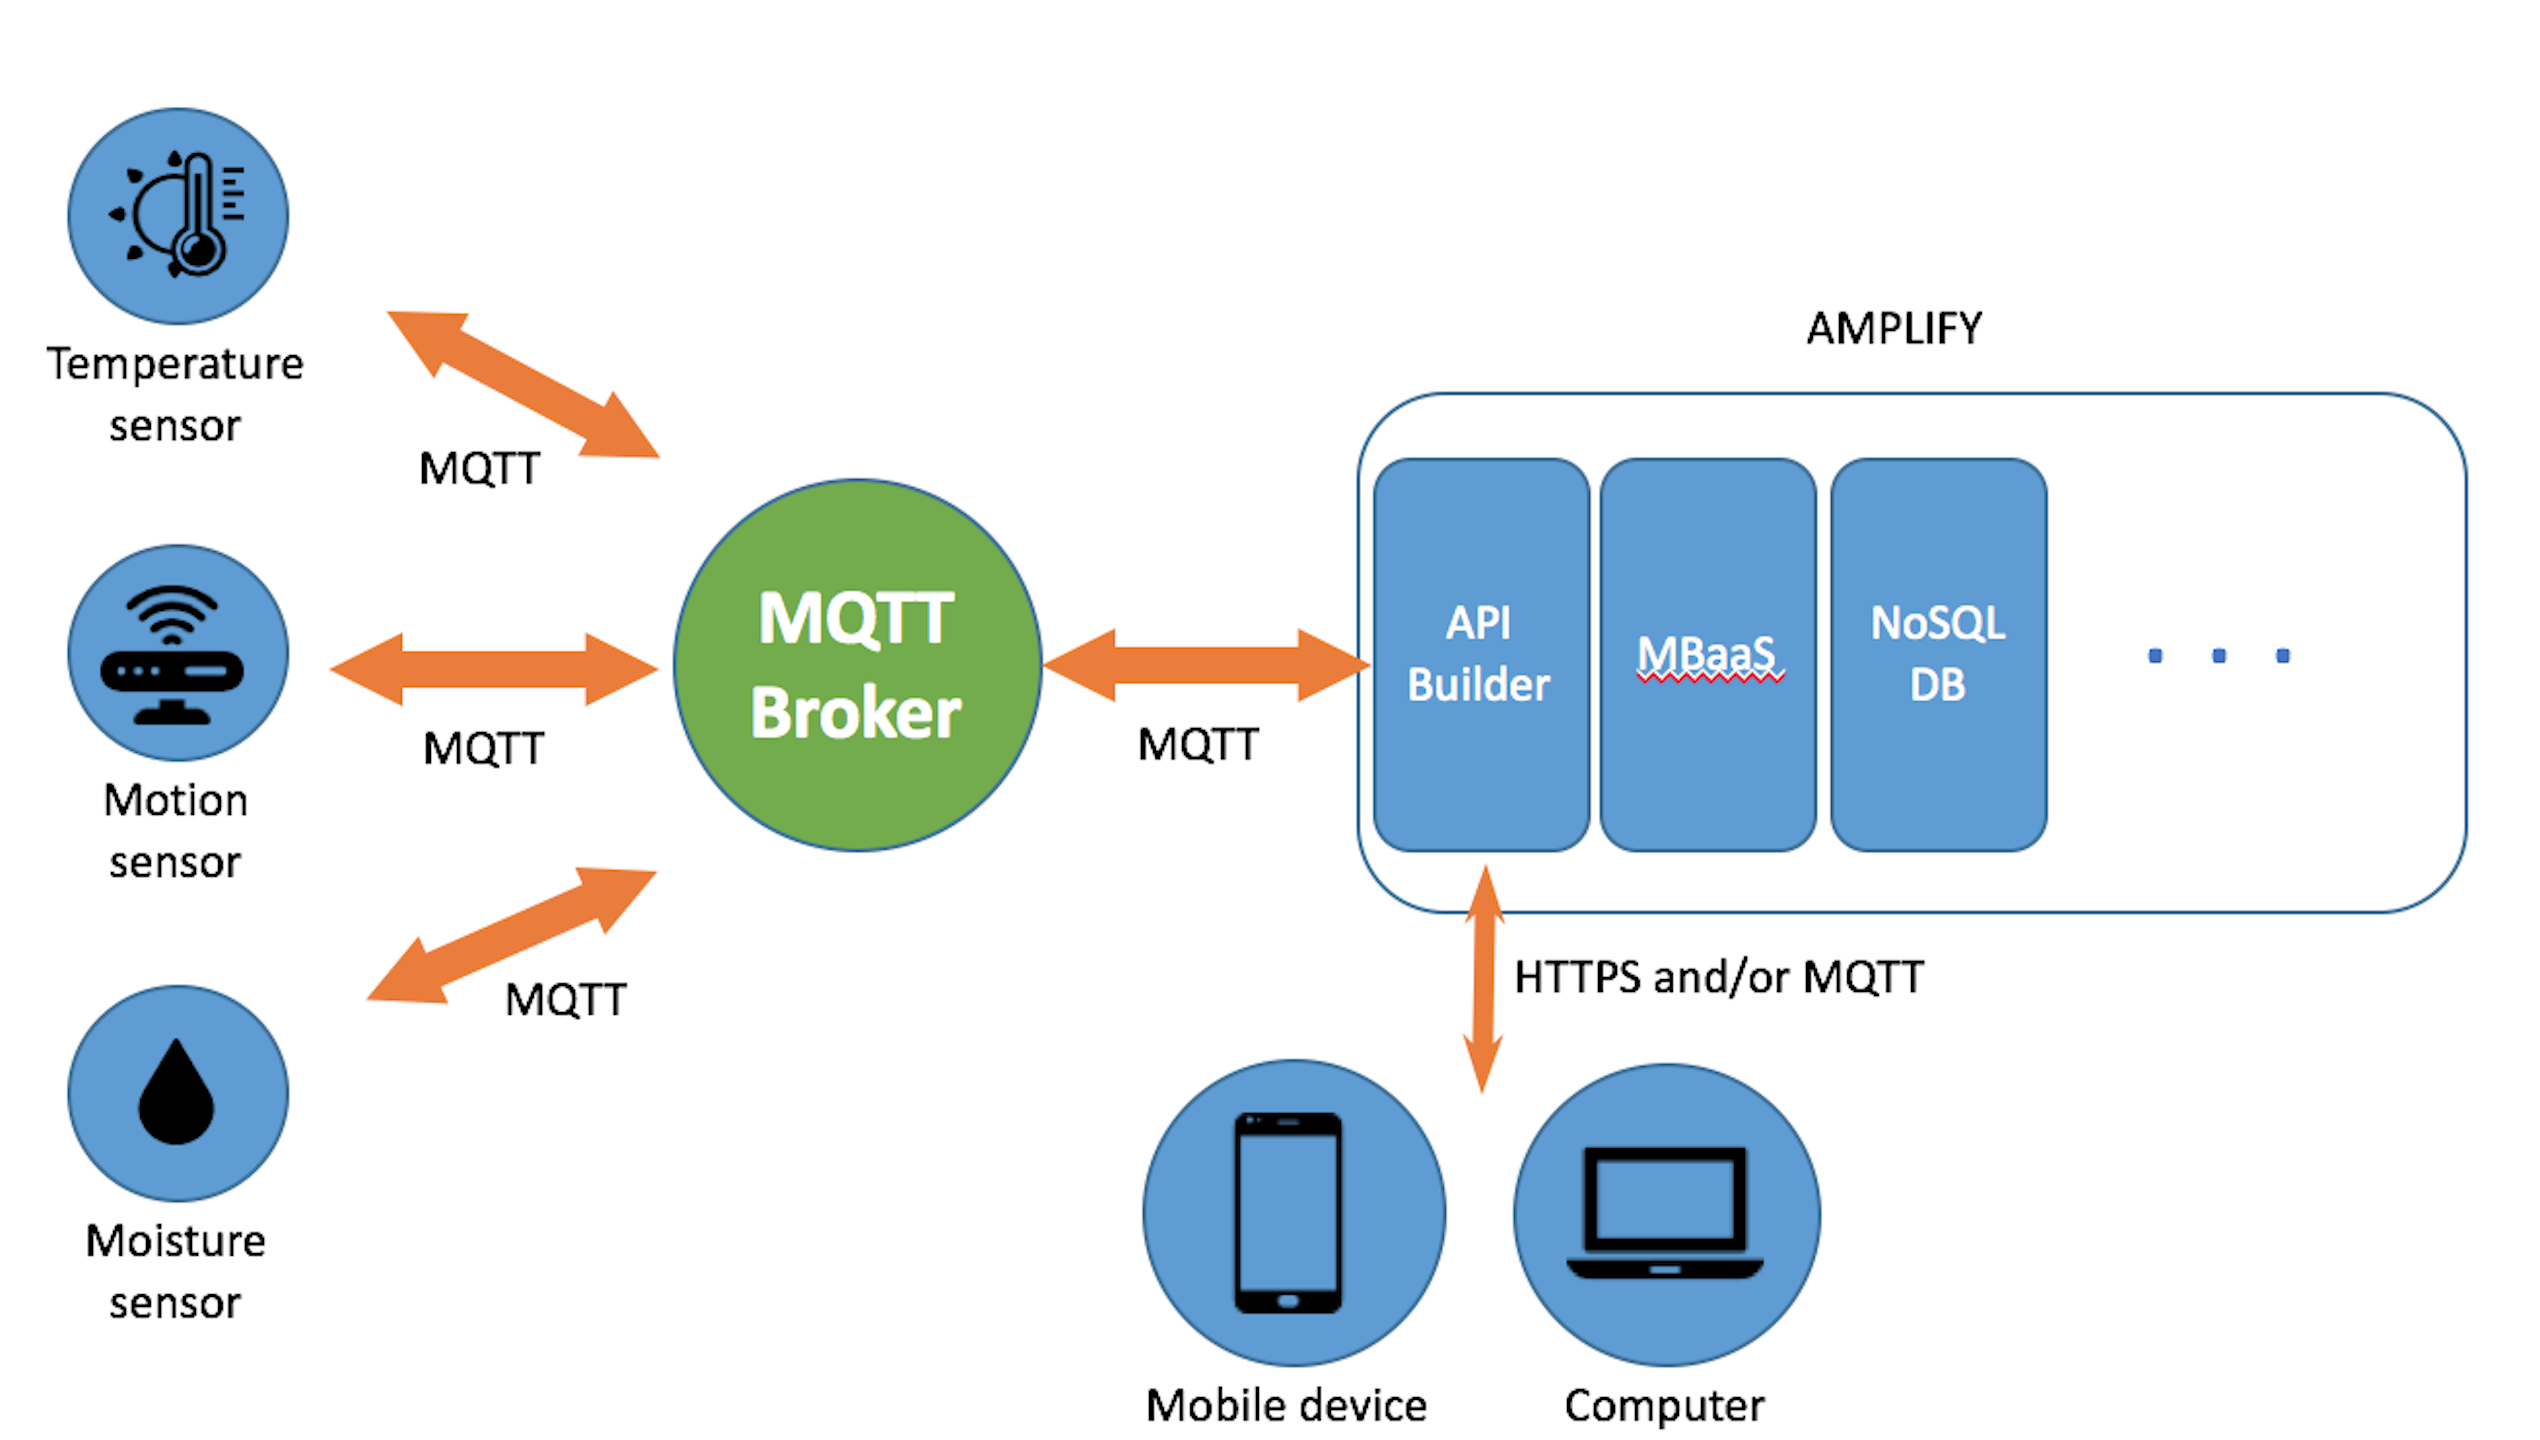
\includegraphics[scale=.09]{images/figure.png}
\caption{this is a picture}
\label{fig:1}
\end{figure}


\section{Your proposal (Concept)}
\label{sec:3}
   What is your project?
\\ requirements table
\\ Add a picture explaining how it works (concept)
\\ Diagrams
\\

\section{Implementation of your proposal}
\label{sec:4}
   if you have class diagram
\\ or an image that show parts of your system
\\ screenshots of part of your code
\\ explain the main parts of the code
\\ make a relation between the functionalities of the system and the requirements
\\ like: this part of the code does that which is described in the requirement FR1.

\section{Results}
\label{sec:5}
   show what is working
\\ which requirements are not implemented?
\\ what could you have done in a different way?

\section{Conclusion}
\label{sec:5}
...
\\ future work
\chapter{Implementing the server logic}
\label{intro} 


\abstract{
\\ (1 or 2 lines): Give a context of your project
\\(1 line): what is the problem?
\\(2 lines): how are you solving it?
\\(1 or 2): what are the results/conclusions
}

\section{Introduction}
\label{sec:1}


\section{Related works}
\label{sec:2}

The research group BLABLA \cite{cheng2015building} did a similar work....using MQTT as it is shown in Figure \ref{fig:1}.
\begin{figure}
\sidecaption
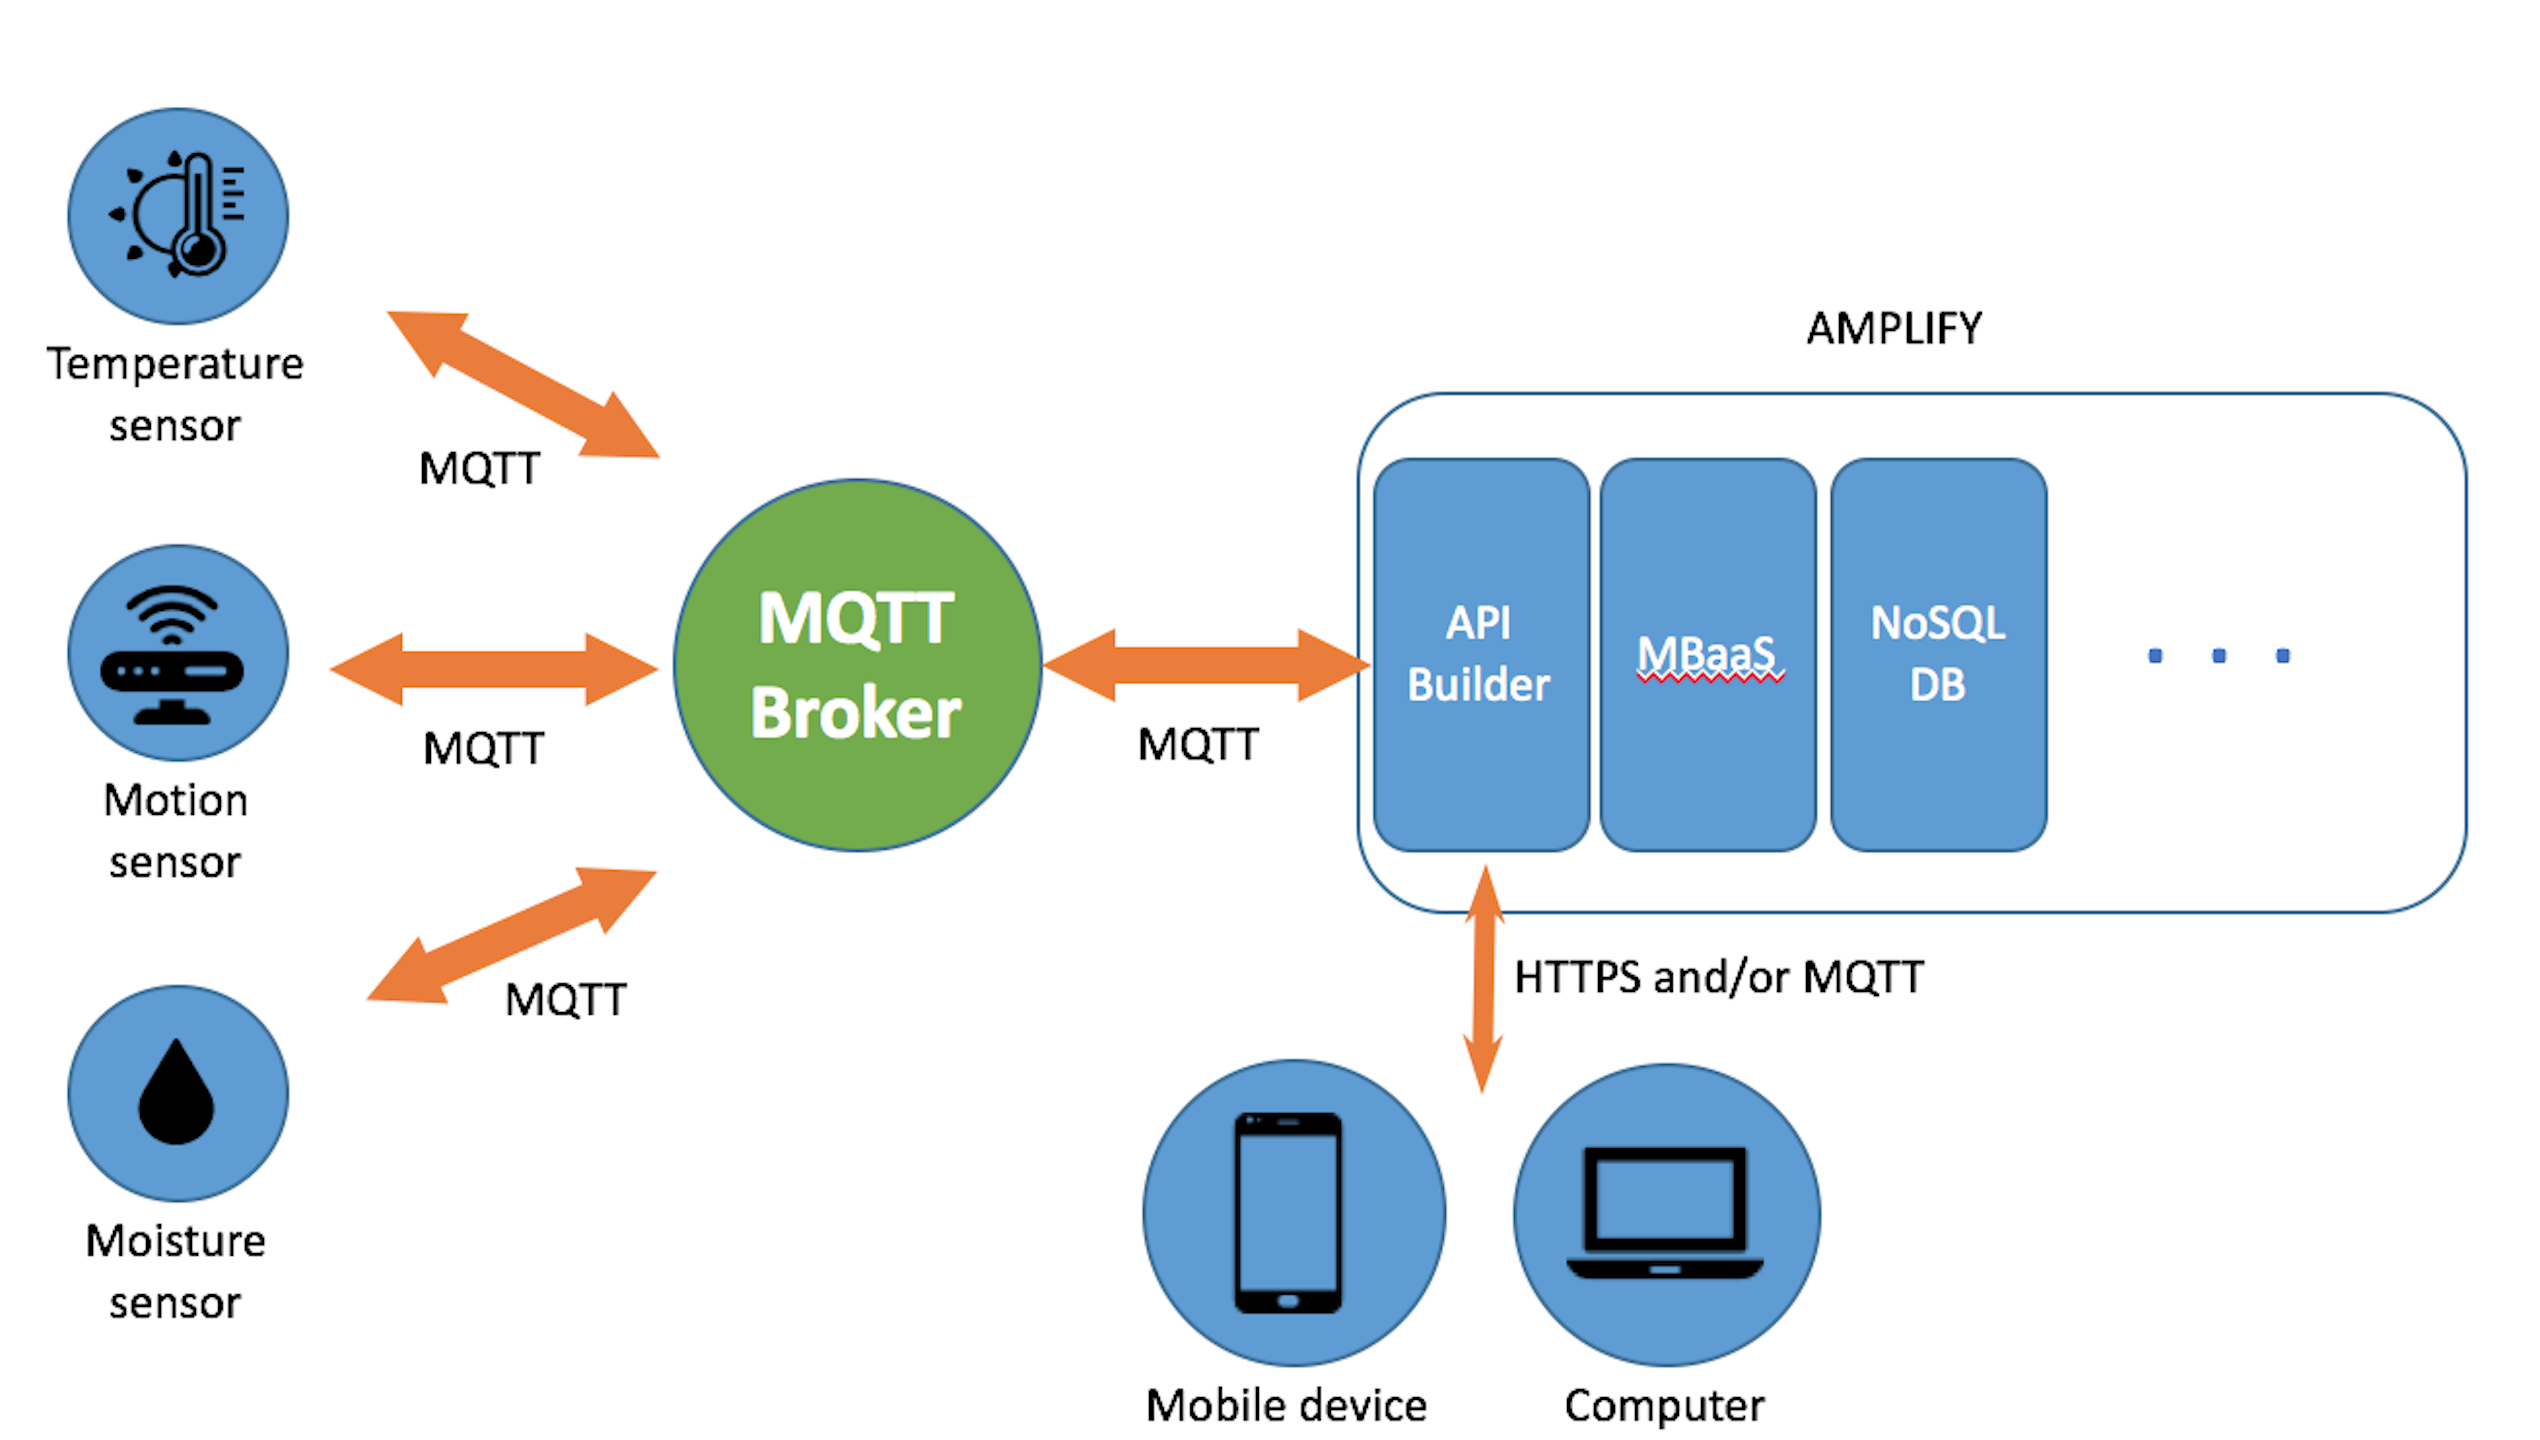
\includegraphics[scale=.09]{images/figure.png}
\caption{this is a picture}
\label{fig:1}
\end{figure}


\section{Your proposal (Concept)}
\label{sec:3}
   What is your project?
\\ requirements table
\\ Add a picture explaining how it works (concept)
\\ Diagrams
\\

\section{Implementation of your proposal}
\label{sec:4}
   if you have class diagram
\\ or an image that show parts of your system
\\ screenshots of part of your code
\\ explain the main parts of the code
\\ make a relation between the functionalities of the system and the requirements
\\ like: this part of the code does that which is described in the requirement FR1.

\section{Results}
\label{sec:5}
   show what is working
\\ which requirements are not implemented?
\\ what could you have done in a different way?

\section{Conclusion}
\label{sec:5}
...
\\ future work
\chapter{Hospitals in Smart Cities}
\label{abstract} 
%\usepackage{booktabs}
%\usepackage{colortbl}
%\usepackage[strings]{underscore}
%\usepackage{pdfpages}
%\usepackage{url}
\textsl{written by \\ Melanie Löbel, \\ Matriculation number 2170582
} \\ \\


\abstract
\\This chapter describes how hospitals are integrated into the "Smart City" project.
In case of an accident it is important to know which hospital is the nearest one and if it has the appropriate specialists. Also it’s important to know if the hospital or the doctor is available.
The main problem is to get those information as soon as possible because it can be essential for survival. For this purpose, each hospital must have its own ID and save the respective data such as location, existing specialists and their availability and transmitted these ones to the server. As soon as the respective hospital is contacted by the server via the corresponding topic, these information can be retrieved.
The implementation was carried out via MQTT (Message Queuing Telemetry Transport). JSON (JavaScript Object Notation) was used for simple and language independent data exchange. Python is used as programming language.

%}

\section{Introduction}
\label{sec:1}
There are a lot of working definitions for a smart city. Washburn et al. defines a smart city in this way: "The use of Smart Computing technologies to make the critical infrastructure components and services of a city - which include city administration, education, healthcare, public safety, real estate, transportation and utilities - more intelligent, interconnected and efficient." \cite{nam2011conceptualizing} In this chapter is described the healthcare in form of making a hospital search more efficient.

\section{Product overview (Context)}
\label{Hospital_Product overview}

%The research group BLABLA \cite{cheng2015building} did a similar work....using MQTT as it is shown in figure \ref{fig:1}.

By using MQTT it has to be guarantee that the hospital is registered to the server, also called the MQTT Broker \cite{zabasta2018mqtt}. Each hospital has its own stored data like location, doctors, availability and so on. The hospital must listen to the server and send the information when the responding topic is called. This happens when a client e.g. a patient is searching for a hospital or specialist. The topic that each hospital has to subscribe is '/hshl/hospitals/hospital_id'. Within this channel the data and messages should be transferred. For sending the relevant data to the server the hospital has to publish the topic '/hshl/hospitals/' too. This procedure results a context of following parts, the MQTT broker as central unit and the recipient represent as a patient and the sender consisting of three hospitals, see figure \ref{Overview environment}. 

\begin{figure}[H]
\centering
\sidecaption
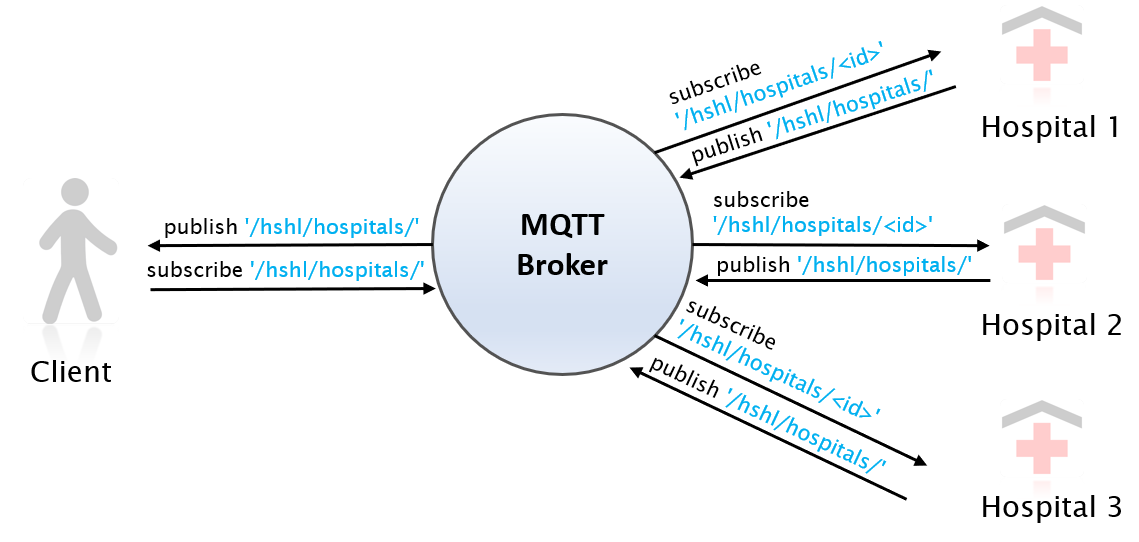
\includegraphics[scale=.375]{images/Bild1-5.png}
\caption{Overview environment and 'topic' for communication}
\label{Overview environment}
\end{figure}

%\clearpage


\section{Concept}
\label{sec:3}
In case of an accident, the person needs help as soon as possible. 
It is important not only that help arrives quickly at the accident site, 
it is also important to know where the nearest hospital is located, 
if it is available and if it has the needed specialist. For that, information such as the name of the hospital, its ID and  GPS coordinates, the number of free rooms and the specialist doctors must be stored, regularly updated and transmitted to the server.
As soon as the hospital is transferred from the server via the respective topic ''/hshl/hospitals/hospital_id'' 
these data should be displayed or sent to the server. 
\\
The patient should be able to make an appointment directly with the respective specialist e.g. in case of a light accident.
So for each doctor there must be saved information data such as specialist fields and available times.
For such function there must be realized a simple usability. The client should be able to choose functions like 'make an appointment' or 'show free rooms'. For that the concept idea is to create a menu item with select options.

%\newpage

\subsection{Requirements}
All these needed information for a hospital results in the following requirements, shown in table \ref{tab_refs}.
%\\

\begin{table}
\centering
\caption{Table of functional (FR) and non functional requirements (NFR)}
\label{tab_refs}
\setlength{\extrarowheight}{0pt}
\addtolength{\extrarowheight}{\aboverulesep}
\addtolength{\extrarowheight}{\belowrulesep}
\setlength{\aboverulesep}{0pt}
\setlength{\belowrulesep}{0pt}
\begin{tabular}{|l|l|} 
\toprule
\multicolumn{2}{|l|}{{\cellcolor[rgb]{0.753,0.753,0.753}}Requirements}                                                                                                                        \\ 
\hline
ID.                                       & Description                                                                         \\ 
\hline
\hline
\rowcolor[rgb]{0.894,0.894,0.894} 
FR 1  & The system must save user data for each hospital.                                      
\\ 
\hline
FR 1.1 & The system must save the name, the ID and the total number of free rooms.                         
\\ 
\hline
\rowcolor[rgb]{0.894,0.894,0.894} 
FR 2  & The system must save location for each hospital via GPS coordinates.               
\\ 
\hline
FR 3  & The system must save medical information about the hospital.                       
\\ 
\hline
\rowcolor[rgb]{0.894,0.894,0.894} 
FR 3.1 & The system must save the medical specialist fields.                              
\\ 
\hline
FR 3.2  & The system must save the number of doctors.                                        
\\ 
\hline
\rowcolor[rgb]{0.894,0.894,0.894} 
FR 3.3   & The system must save number of rooms within each specialist fields and their status, free or taken.         
\\ 
\hline
FR 4 & The system must check availability of doctors.                                                                
\\ 
\hline
\rowcolor[rgb]{0.894,0.894,0.894} 
FR 4.1  & The system must get a request for free appointment of a doctor.                    
\\ 
\hline
FR 4.2  & The system must check the date which was given as input.                           
\\ 
\hline
\rowcolor[rgb]{0.894,0.894,0.894} 
FR 4.2.1 & The system must check if the input date is an available date (today or in future) and if it is a weekday.    
\\ 
\hline
FR 4.3 & The system must send a message which times are available for the respective doctor.                           
\\ 
\hline
\rowcolor[rgb]{0.894,0.894,0.894} 
FR 4.4 & The system must check the time which was given as input.                           
\\ 
\hline
FR 4.4.1 & The system must check if the input time for the respective date and doctor is free.                           
\\ 
\hline
\rowcolor[rgb]{0.894,0.894,0.894} 
FR 4.5 & The system must save the appointment with patient name, date and time into the calendar from the respective doctor.  
\\ 
\hline
FR 4.6 & The system must send a message info "Accepted appointment".                                                   
\\ 
\hline
\rowcolor[rgb]{0.894,0.894,0.894} 
FR 5  & The system must check availability of rooms in a medical specialist field.                                  
\\ 
\hline
FR 5.1  & The system must get a request for availability in one medical specialist field.                             
\\ 
\hline
\rowcolor[rgb]{0.894,0.894,0.894} 
FR 5.2  & The system must send a message how many rooms are free or if there is no room available.                      
\\
\hline
FR 6  & The system must register to the server, the MQTT Broker.                      
\\
\hline
\rowcolor[rgb]{0.894,0.894,0.894} 
FR 7  & The system must listen to messages from the server.                      
\\
\hline
FR 8  & The system must send messages like the hospital info to the server.                      
\\
\hline
\hline
 

NFR 1 & Usability                                                                                                     
\\ 
\hline
\rowcolor[rgb]{0.894,0.894,0.894} 
NFR 1.1  & Menu item to choose between options like "Show free rooms", "Show specialists" and "Make an appointment".     
\\ 
\hline
NFR 2  & Efficiency                                                                                                    
\\ 
\hline
\rowcolor[rgb]{0.894,0.894,0.894} 
NFR 3 & Performance                                                                                                   
\\ 
\hline
NFR 3.1 & Guarantee that each message is received only once by the intended recipients: QoS (Quality of service) level 2                                                                                        
\\
\hline
\rowcolor[rgb]{0.894,0.894,0.894} 
NFR 3.2 & Usage of a simple and language independent data exchange format: JSON (Java Script Object Notification)                                                                                         
\\
\hline
NFR 4  & Privacy protection                                                                                             
\\ 
\hline
\rowcolor[rgb]{0.894,0.894,0.894} 
NFR 5  & Safety                                                                                                        
\\
\bottomrule
\end{tabular}
\end{table}
\newpage
\subsection{Use Case Description}
The functional requirements indicate the following use case, how the system should work with the hospital as actuator.
The hospital must be registered with the server with its own ID. In addition, the hospital has to store local information and medical data. The medical data must be updated regularly. This includes the doctors with their specialist fields and their availability regarding of free appointments. Also the availability of the hospital is needed in form of the number of free rooms. All these data should be transferred to the subscriber if the responding topic is called.
In addition the hospital should include the option to make appointments directly with the respective specialist. In case of an only light accident. For this the hospital must check the available appointments for the selected specialist when an appointment request arrives.
Depending on the availability of the appointment, the hospital should accept or reject the appointment, see figure \ref{Use_Case}.
\\

\begin{figure}[H]
\centering
\sidecaption
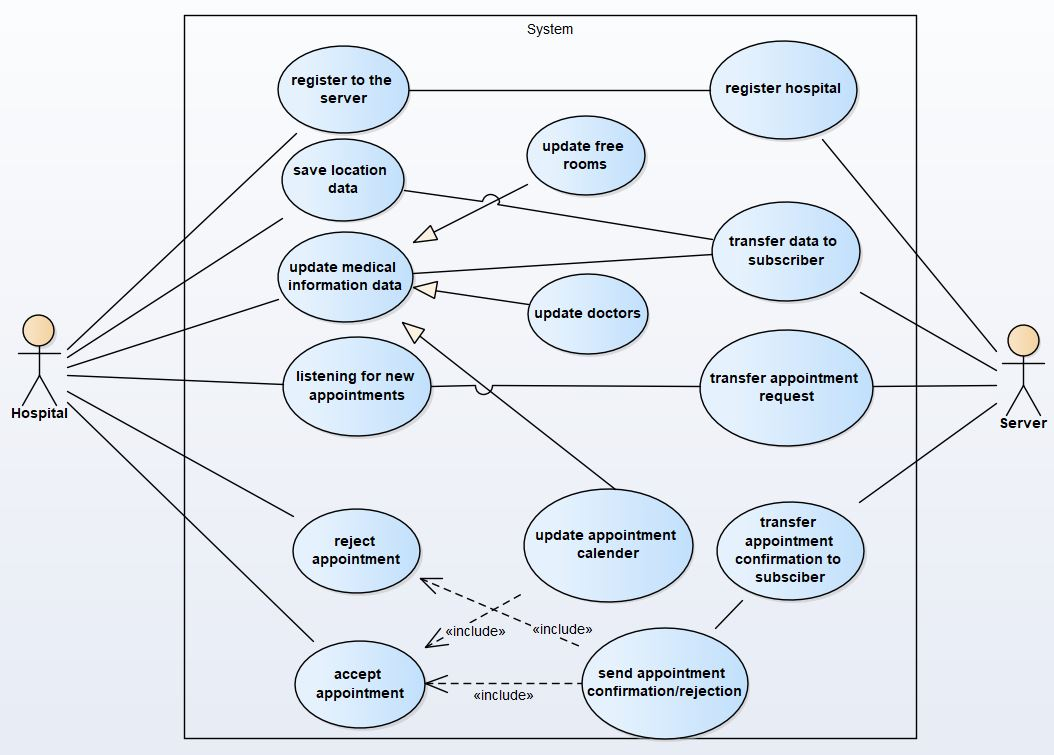
\includegraphics[scale=.425]{images/UseCase_Hospital-Search_variant-2.jpg}
\caption{Use Case Diagram}
\label{Use_Case}
\end{figure}

%For this procedure instruction it is shown in the follow class model  a concept of building up the classes following %data has to be stored in following classes

%\\ Add a picture explaining how it works (concept)
%\\ Diagrams
\\
\clearpage
\section{Implementation}
\label{sec:4}

After definition of the functional requirements and the use case, the object-oriented analysis followed to find the individual classes with attributes and necessary functions. 
A hospital has a name, an ID, a GPS location via coordinates and a number of free rooms. In addition, each hospital has several doctors. They have a title, a name, and a phone number. Each doctor is a specialist in one or more fields. In addition, every doctor is available at certain times on weekdays. That can be in the morning and/or in the afternoon. The doctors with their specialist fields, the number of free rooms and all busy appointments are to be displayed via a query. In addition, an appointment with a doctor should be able to be arranged with a date and time. Appointments are only compatible on weekdays and in the future. In case of an accident and for the search for a suitable hospital nearby, the server must have the following data: name of the hospital, the ID, the GPS location, the number of doctors and free rooms and the specialist fields of all doctors, in order to have the respective specialist depending on the type of an accident. These data has to be stored in one message which has to be transmitted to the server via JSON format. 
For the required communication to the server there should be a separate class 'Communication' implemented which contains the topic with all necessary methods for MQTT communication. So the class 'Communication' should ensure that the hospital communicates via publish and subscribe the respective topic. 
In following figure \ref{Class_diagram} the different classes with their needed attributes and methods are simply described.

\begin{figure}[H]
\centering
\sidecaption
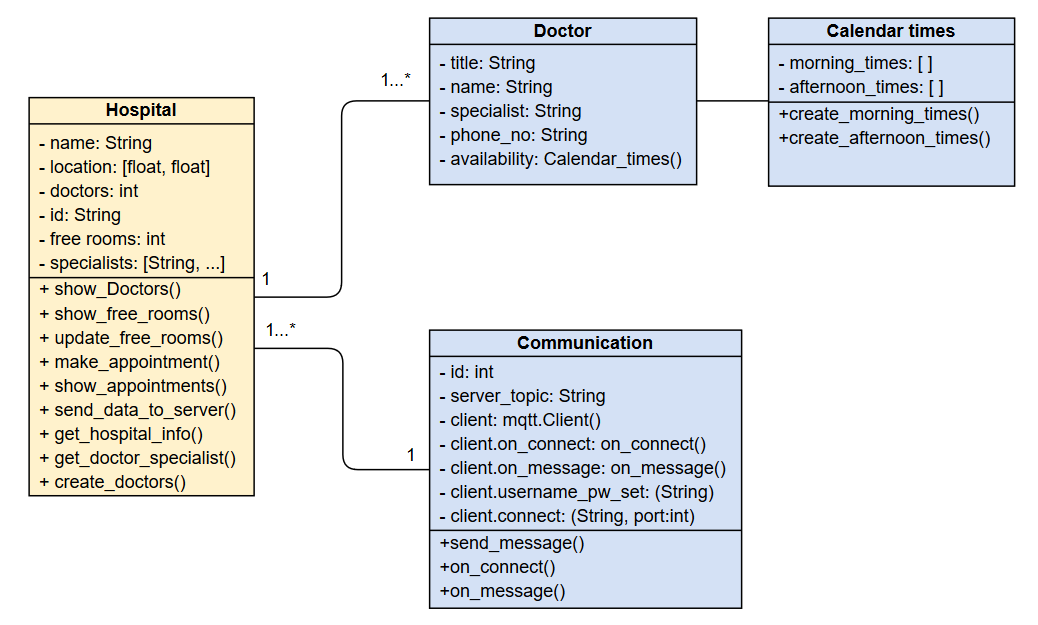
\includegraphics[scale=.425]{images/Class_model.png}
\caption{Class Diagram}
\label{Class_diagram}
\end{figure}

\\
\subsection{Classes with relation to requirements}
\subsubsection{Communication}
Important for the MQTT communication is to import the mqtt client, see figure \ref{Communication} line 1. For using the JSON data exchange (NFR 3.2) json has to be imported too. For the procedure to make an appointment with the doctor the package time has to be imported. Next to the topic '/hshl/hospitals/' the connect and message event must be also assigned. In addition the user name, the password and the broker address is needed to connect with it (FR 6). For listening to the server the method 'on_connect' is needed (FR 7). For sending a message the methods 'send_message' and 'on_message' must be included (FR 8). The hospital is only response when it is directly selected about the topic and its self.id. The relevant data will be send as a message in JSON format about the general topic '/hshl/hospitals/', see line 23 in figure \ref{Communication}.

\begin{figure}[H]
\centering
\sidecaption
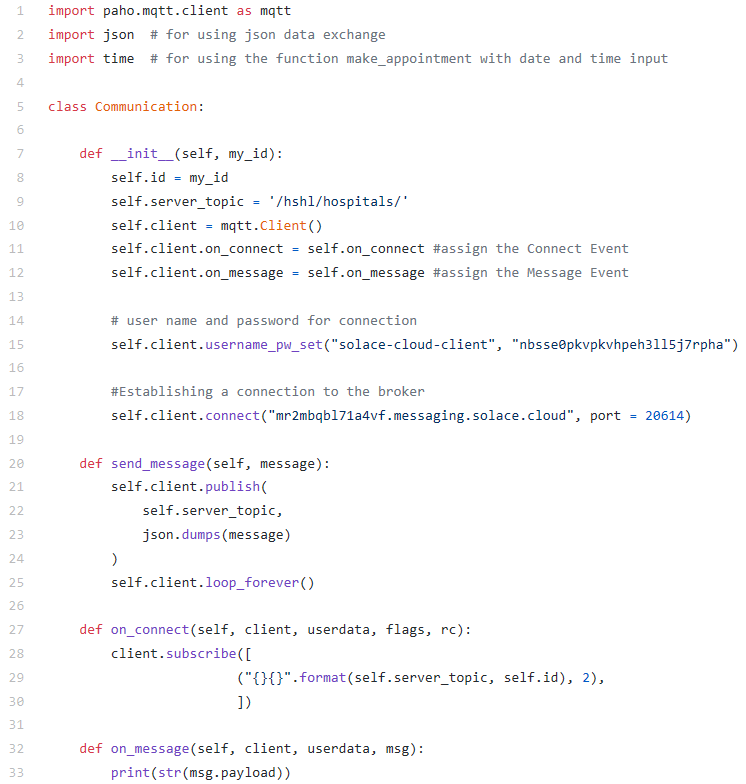
\includegraphics[scale=.53]{images/Communication.png}
\caption{Class Communication}
\label{Communication}
\end{figure}

In line 29 in figure \ref{Communication} the QoS level is set to '2' like required with NFR 3.1. It is the highest level of service in MQTT. This level guarantees that each message is received only once by the intended recipients. QoS 2 is the safest and slowest quality of service level. The guarantee is provided by at least two request/response flows (a four-part handshake) between the sender and the receiver \cite{ferguson1998quality}.

\subsubsection{Doctor and Calendar times}
In the class Doctor it's only necessary to create the constructor with the needed attributes like described in the class diagram in figure \ref{Class_diagram}. Important is that here are two methods. One method for returning the title, name and specialist field from the doctor as info string and the other method for representation or displaying it. 

\begin{figure}[H]
\centering
\sidecaption
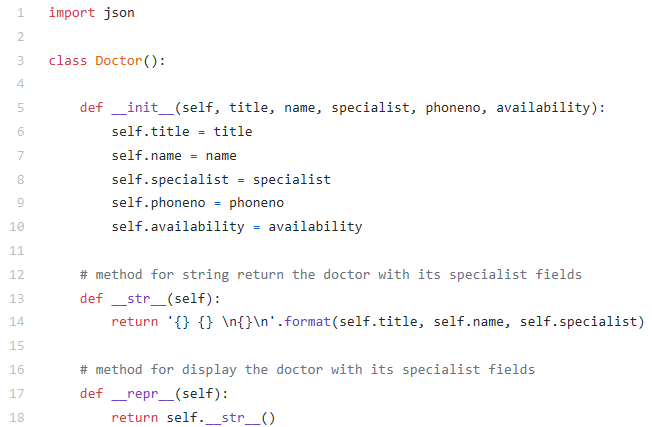
\includegraphics[scale=.65]{images/Doctor.png}
\caption{Class Doctor}
\label{Doctor}
\end{figure}

The next important class which affects the appointment making is 'Calendar times'. It contains the available times when a doctor would be available. It's separated in morning and afternoon times. Later in the hospital class a doctor can be created as a new object which has both available times in the morning and in the afternoon or only one of it. Important is here to import datetime.

%\begin{figure}[H]
%\centering
%\sidecaption
%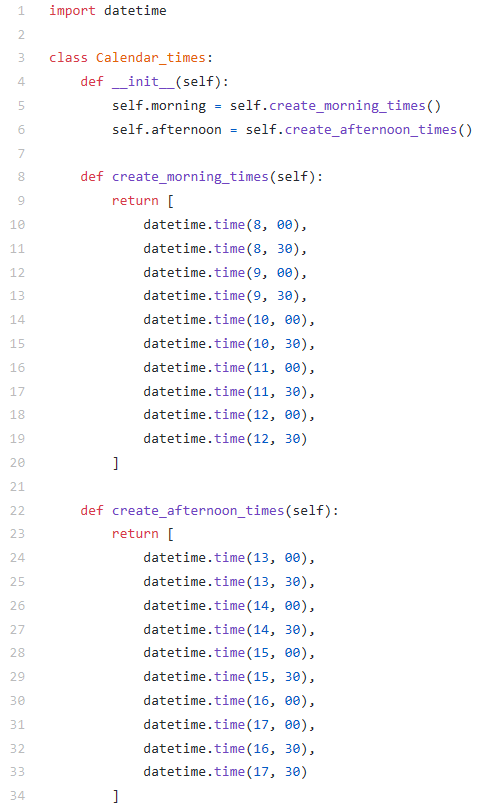
\includegraphics[scale=.65]{images/Calendar_times.png}
%\caption{Available calendar times}
%\label{Calendar_times}
%\end{figure}

\begin{figure}[t]
\begin{minipage}[t]{0.475\textwidth}
\centering
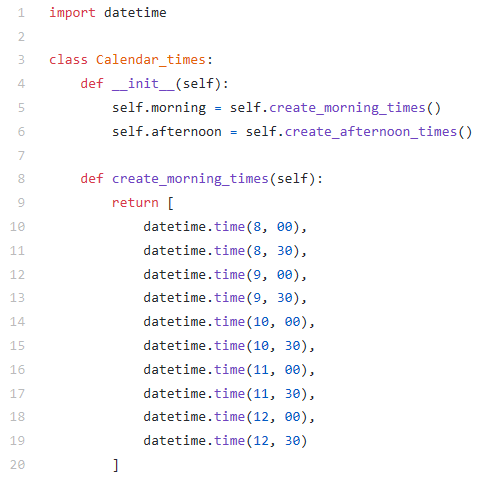
\includegraphics[scale=.65]{images/Calendar_times-1.png}
    \caption{Available calendar times}
    \label{Calendar_times}
\end{minipage}
\hfill
\begin{minipage}[t]{0.475\textwidth}
\centering
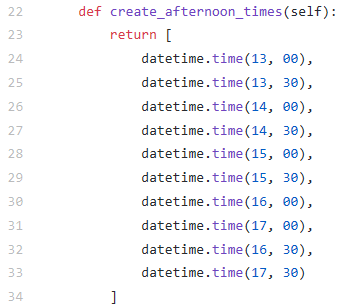
\includegraphics[scale=.65]{images/Calendar_times-2.png}
    %\caption{2}
    \label{2}
\end{minipage}
\end{figure}

\subsubsection{Hospital}
The main important class is the hospital. The other classes like Communication, Doctor and Calendar times has to be imported into the class Hospital. In addition for make an appointment also the packages datetime and calendar are needed to be imported. In figure \ref{hospital_attributes} is represented the needed attributes which are required in FR1, FR2, FR3.1, FR3.2, FR4.5.

\begin{figure}[H]
\centering
\sidecaption
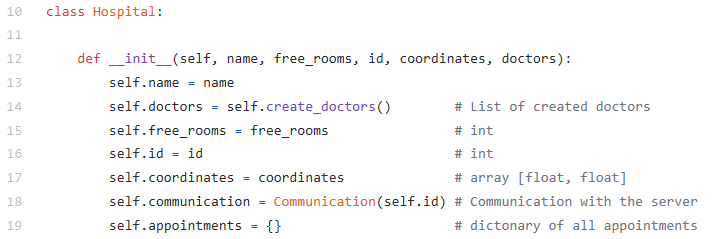
\includegraphics[scale=.65]{images/Relevant_attributes_in_the_hopital_class.png}
\caption{Needed attributes in the class Hospital}
\label{hospital_attributes}
\end{figure}


In the project 'Smart City' the main requirement is that the attributes which are shown in figure \ref{Relevant_attributes_server} in the dictionary 'hospital_info' will be send to the server. Including name and location coordinates of a hospital, the total number of doctors, the hospital ID, the total number of free rooms and the specialist fields. So the first step is to get these data and stored it into 'hospital info' as a dictionary. This structure is necessary for sending data in JSON format \cite{sporny2019json}. Also it is relevant return this hospital info so that another method have access to this info, see line 184 in figure \ref{Relevant_attributes_server}. 

\begin{figure}[H]
\centering
\sidecaption
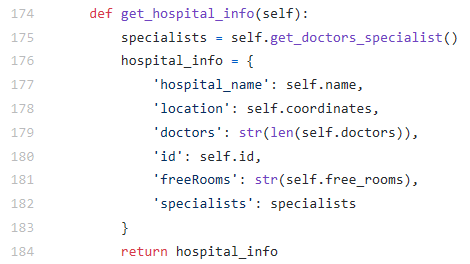
\includegraphics[scale=.65]{images/get_hospital_info.png}
\caption{Relevant attributes for the server}
\label{Relevant_attributes_server}
\end{figure}

With the variable 'message' the hospital info will be saved about the access on method self.get_hospital_info(). Afterwards this message will be send to the server with the access to the class Communication, see line 172 in figure \ref{send_hosp_info}. 


\begin{figure}[H]
\centering
\sidecaption
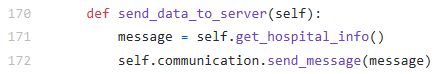
\includegraphics[scale=.7]{images/send_hospital_info.png}
\caption{Data transfer method for sending to the server}
\label{send_hosp_info}
\end{figure}

Like in introduction in subsection \ref{tab_refs} described it should be also feasible to make an appointment with a doctor itself, see requirement FR4. The activity diagram in figure \ref{Make_Appointment} shows how this requirement with its sub requirements are implemented. It's represented the single steps until the appointment is accepted. So after a date is entered it will be check if it is a weekend or if this date is in the past. For these both situation a new date has to be entered. It's realized with an if and elif condition. If both situation are not true the else condition continues and a request for a time will be send. The next step is to check if the entered time is available for this date with the respective doctor. For that all appointments has to be summarized in a dictionary.

\begin{figure}[H]
\centering
\sidecaption
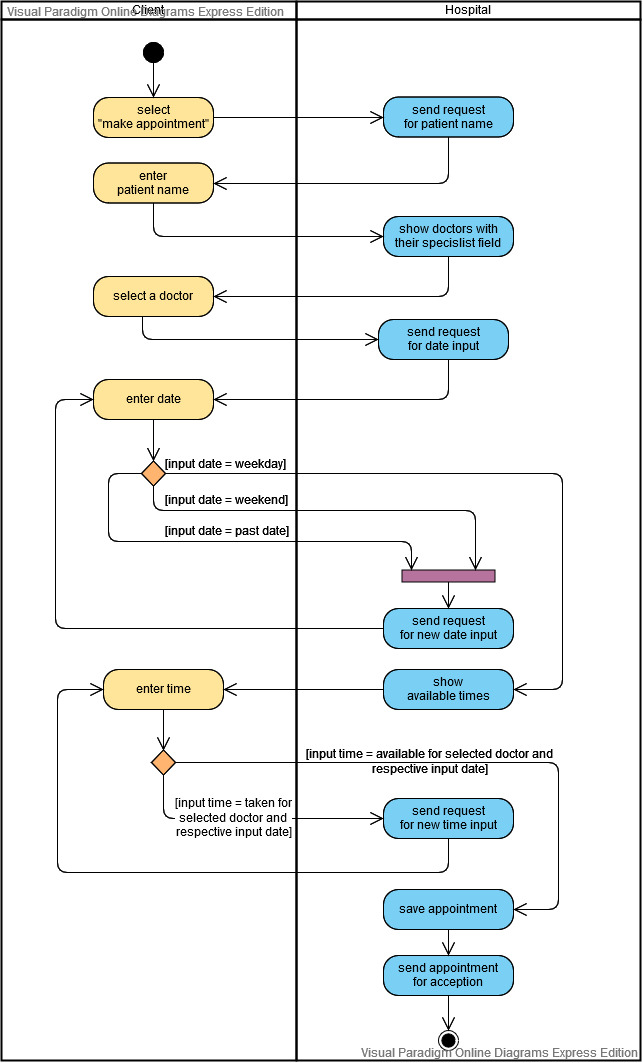
\includegraphics[scale=.55]{images/MakeAppointment.jpg}
\caption{Activity Diagram "make an appointment"}
\label{Make_Appointment}
\end{figure}

For being sure that a room is available when it's needed there will be a room reserved in condition that an appointment is accepted. An info message for this is sent and the number of rooms will be adapt. %, see cut out of the code in the hospital.py, figure \ref{Acception}.

%\begin{figure}[H]
%\centering
%\sidecaption
%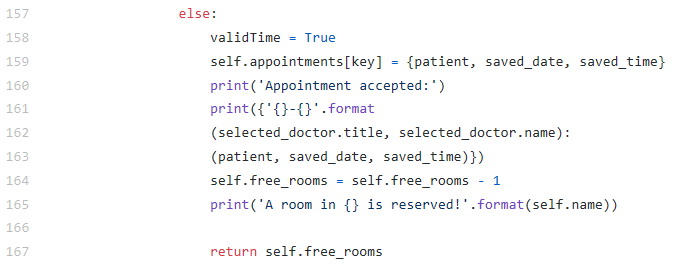
\includegraphics[scale=.65]{images/Acception.png}
%\caption{Acceptation message of an appointment with room reservation }
%\label{Acception}
%\end{figure}

\subsubsection{Usability}
To have something like an overview about the main functions the non functional requirement NFR 1.1 was to have a menu item with the possibility to choose options like 'make an appointment' or 'show free rooms'. The possible options or functions which were implemented are described in figure \ref{Options}. It shows a cut out of the class Hospital.

\begin{figure}[H]
\centering
\sidecaption
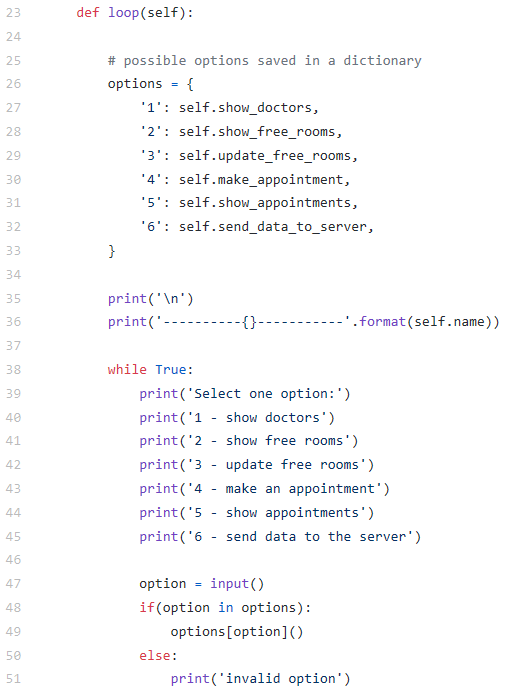
\includegraphics[scale=.65]{images/Options.png}
\caption{Implementation menu item}
\label{Options}
\end{figure}

The functions 'make an appointment' and 'send data to the server' were described in more detail in the sub sections before. the other four functions are very simply in the implementation. It contains only the output via 'print' so that the info is displayed directly. With 'update free rooms' there is the possibility to save a new number via input() of rooms.

\subsubsection{Realization of three hospitals}
Like described in the beginning of this capture in the product overview \ref{Hospital_Product overview} there should be three hospitals. To implement more than one hospital in a smart city there were implemented three additional files: main1.py, main2.py and main3.py.
Here the object Hospital from the class hopital.py is imported. Also the objects Doctor and Calendar_times are needed. So that e.g. in each main.py the respective hospital with its doctors can be initialized.

\section{Results}
\label{sec:5}
In summary the most of the requirements were implemented. This concerns the functional ones FR 1 until FR 4 and FR 6 until FR 8. The sub requirement FR 3.3 were implemented only partly. Only the total number of free rooms were considered and not for each medical specialist field. In condition to that also FR5 with the availability check for each medical specialist field is not full implemented.  But it would be possible to do this in future work with creation of medical stages in each hospital which have a number of rooms. So the code is extendable. In view of the non functional requirements the NFR 1, the usability was full filled with the different select able options. Like described NFR 3 was implemented by setting the QoS level 2 and by using JSON format. The privacy protection described in NFR 4 was already implemented e.g. in hospital.py with the method 'def __init__()'. This format defines a private method. The safety with NFR 5 isn't implemented yet. To increase the efficiency which is required in NFR 2 the function 'make_appointment' could be improved. The function could be adapted in that way that only the times for each doctor will be shown which are free at the chosen date. Currently all times from the doctor are shown. If a time is selected which is taken for the chosen date an info message is send to choose another time. This procedure can be avoid if only the valid times for the chosen date are displayed.
\\

\section{Conclusion}
\label{sec:5}
This capture showed in detail how a hospital could be implemented in the project 'Smart city'. It was given an overview about the requirements and how they were implemented into a python code including usage of MQTT and JSON data transfer. The python code is find below following link \url{https://github.com/melanieloebel/Interaktionskonzept_ITD_MelanieLoebel.git}. The hospital could be upgraded in future work. For example with an emergency room. So that in case of an hard accident this room can be reserved.

\newpage
\bibliographystyle{IEEEtran}
\bibliography{chapter3.bib}

\chapter{Public services in Smart Cities}
\label{intro} 


\abstract{
\\ (1 or 2 lines): Give a context of your project
\\(1 line): what is the problem?
\\(2 lines): how are you solving it?
\\(1 or 2): what are the results/conclusions
}

\section{Introduction}
\label{sec:1}


\section{Related works}
\label{sec:2}

The research group BLABLA \cite{cheng2015building} did a similar work....using MQTT as it is shown in Figure \ref{fig:1}.
\begin{figure}
\sidecaption
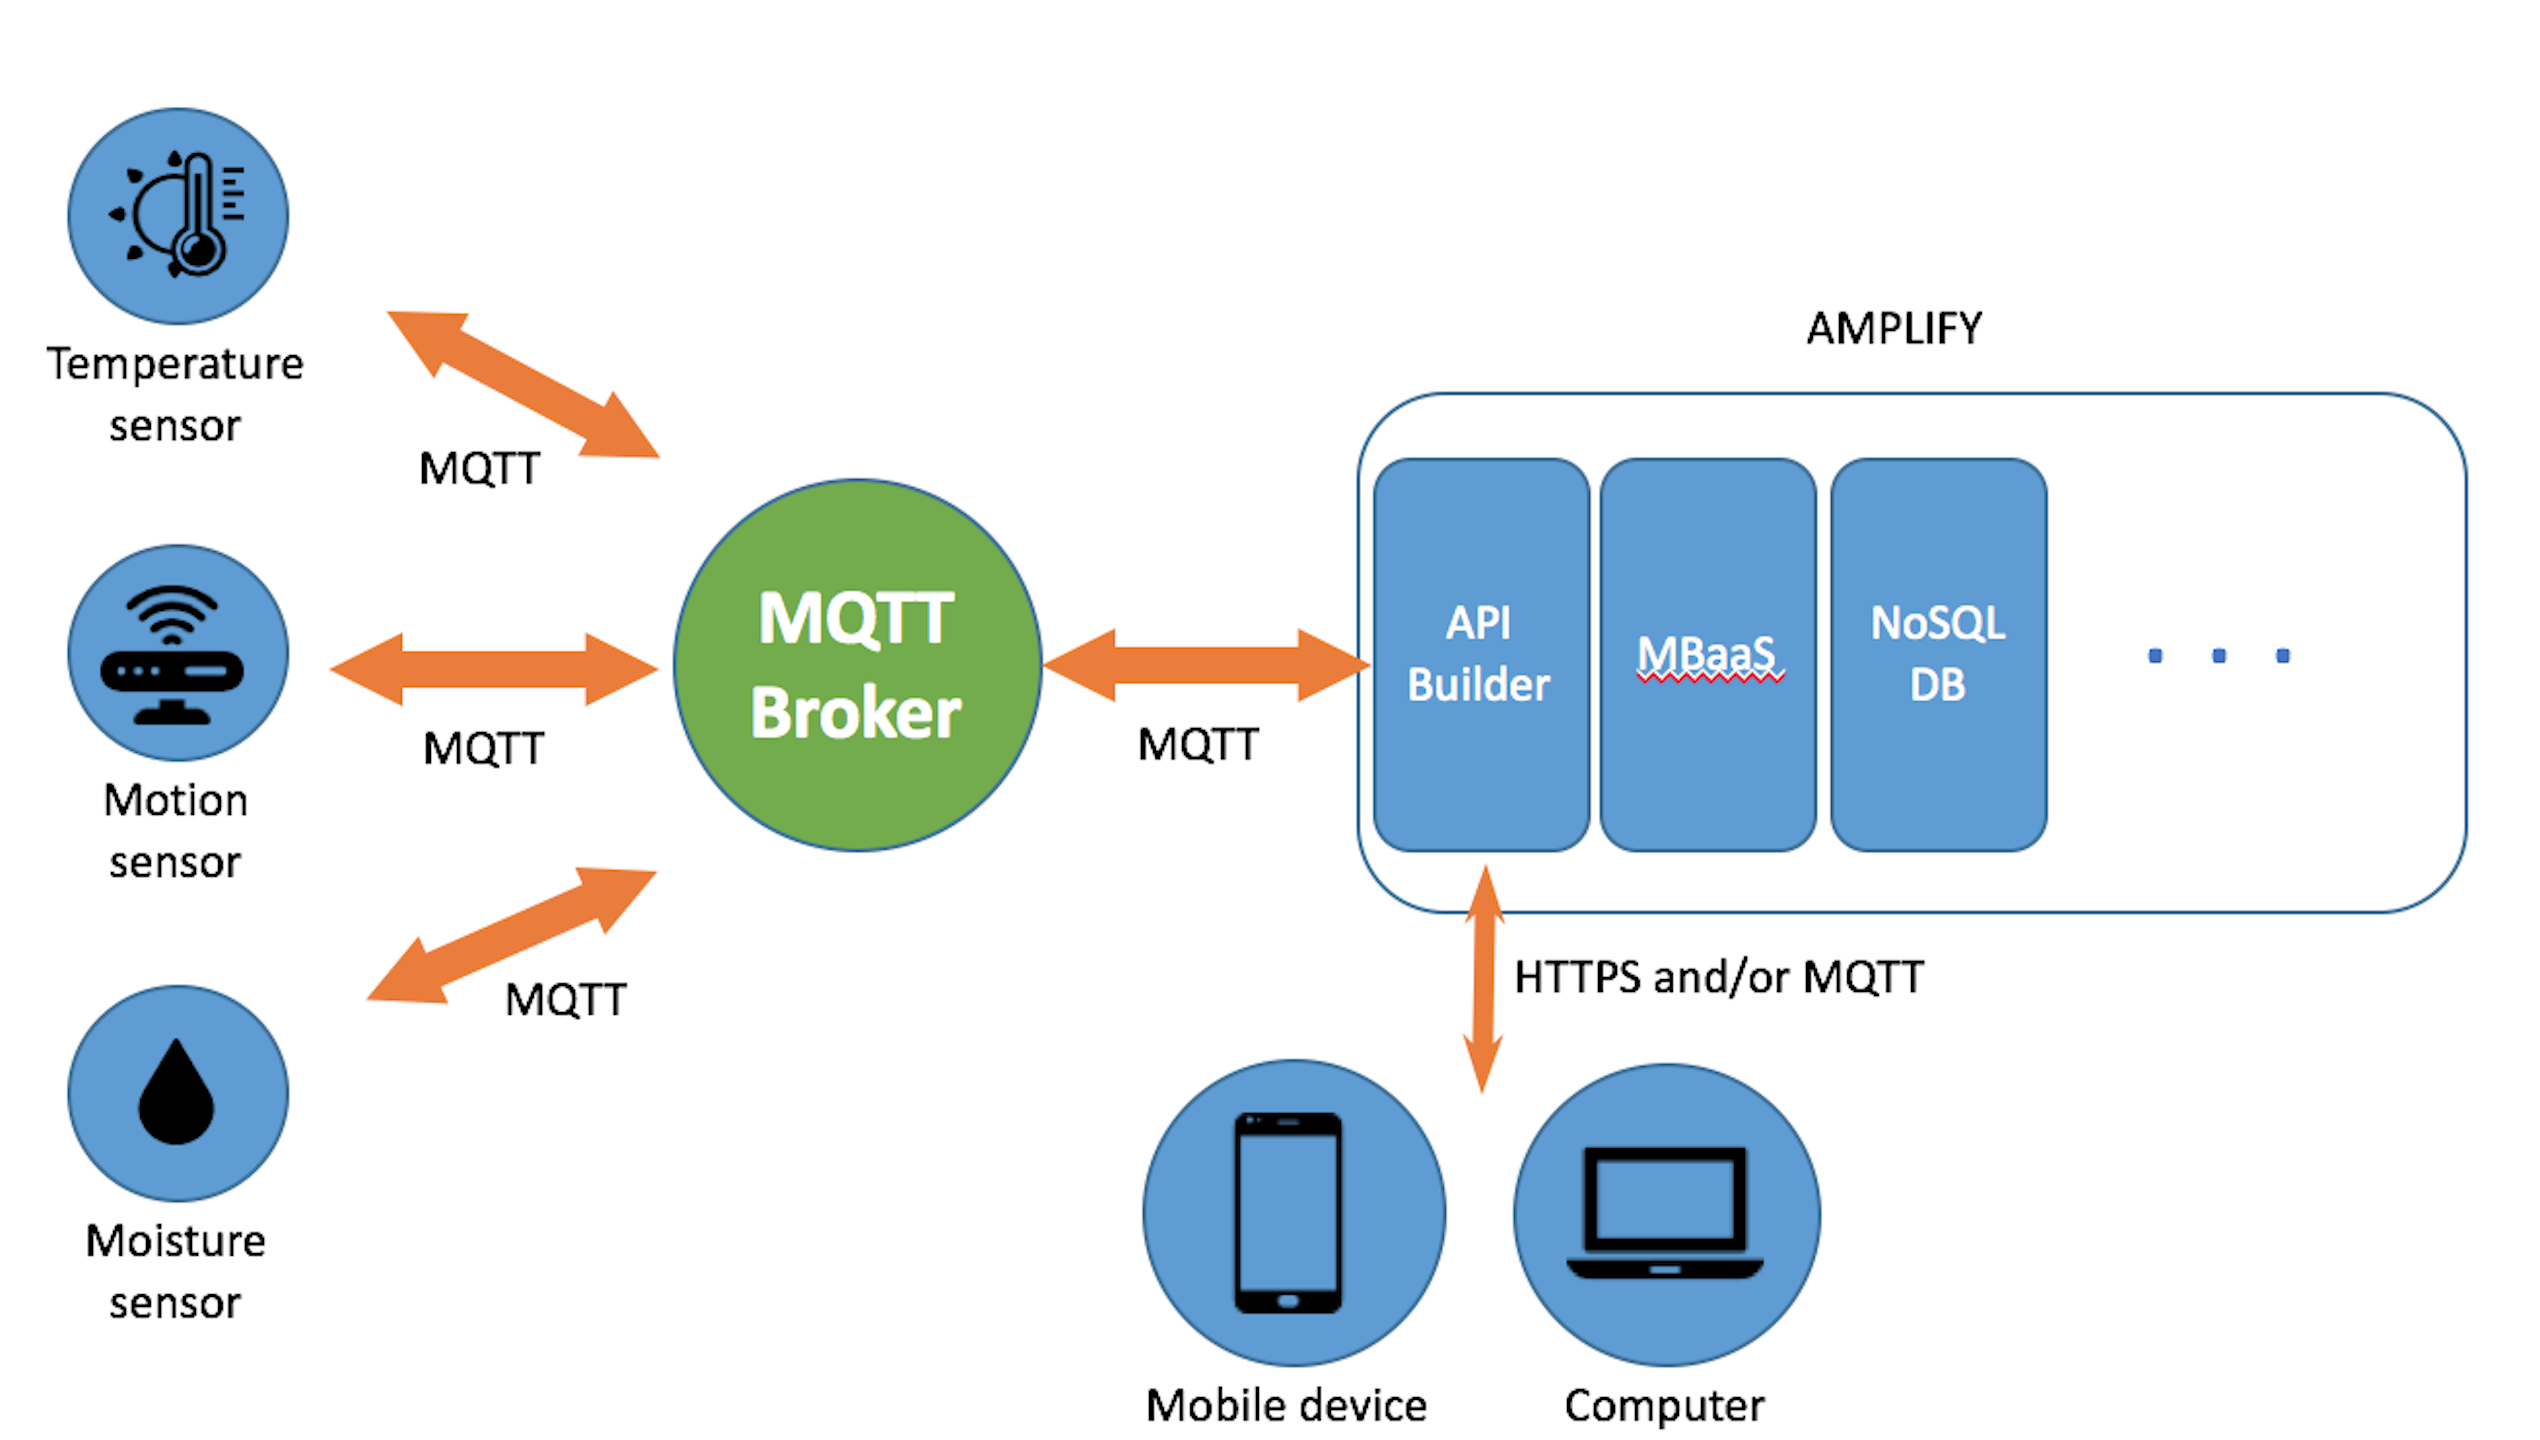
\includegraphics[scale=.09]{images/figure.png}
\caption{this is a picture}
\label{fig:1}
\end{figure}


\section{Your proposal (Concept)}
\label{sec:3}
   What is your project?
\\ requirements table
\\ Add a picture explaining how it works (concept)
\\ Diagrams
\\

\section{Implementation of your proposal}
\label{sec:4}
   if you have class diagram
\\ or an image that show parts of your system
\\ screenshots of part of your code
\\ explain the main parts of the code
\\ make a relation between the functionalities of the system and the requirements
\\ like: this part of the code does that which is described in the requirement FR1.

\section{Results}
\label{sec:5}
   show what is working
\\ which requirements are not implemented?
\\ what could you have done in a different way?

\section{Conclusion}
\label{sec:5}
...
\\ future work
\documentclass{article}
\usepackage[utf8]{inputenc}

\usepackage{graphicx} %package to manage images
\graphicspath{ {./Bilder/} }

\usepackage[rightcaption]{sidecap}

\usepackage{wrapfig}

\title{Service Vehicles Network}
\author{Lukas.Ostrzinski }
\date{June 2020}

\begin{document}

\maketitle

\section{Introduction}

\subsection{Motivation}
Smart Cities is an futuristic concept which has become more and more relevant recently. Because of this, infrastructure like transportation or emergency systems will become more automatic and controlled over an whole server system. 
\newline
Barcelona has always been included in the top 10 rankings when it comes to Smart cities. It has a well-documented history in this area and today integrates intelligent sensors and big data analyzed in a wide variety of areas, from parking lot management and traffic management to garbage disposal, management of air quality and irrigation of green areas. [1]

\subsection{Emergency Services in Smart Cities}
If police, firefighters and ambulances could use this technology, it would be a lot easier for them to react to an emergency like an car crash or other kinds of emergency situations. Automation could make the process of calling an ambulance more efficient and faster. For example, a car which was involved in an car crash could call the ambulance automatically. This would be especially helpful when the driver cannot call the ambulance because he is unconscious or unable to access his phone.




\section{Concept}
The aim of the project is to implement an program which queries the position of an emergency and the type of emergency. Depending on the type of the emergency, the program sends the right vehicle to the position. 
There are 3 kinds of vehicles: ambulances, firetrucks and police cars.
\newline
The program gets the information about the position and the type of the emergency from a server. The program tells the server when it sends the requested vehicle to the location of the emergency and again when the vehicles arrive and leave this location. 

\clearpage
My idea to implement my part of the system was to write 3 programs in which each of them take cares of one of the emergency response vehicles: police cars, firetrucks and ambulances. The structure of each one will be only minimally different. First, I will describe the functional requirements.
\newline
Firstly, the program needs to get the information about the coordinates from the place of operation and determine which of these vehicles needs to be sent to this place. When the program gets this information, it will send an conformation back to the server and say that the vehicle will drive to the place operation. 
\newline

\begin{figure}[htp]
    \centering
\includegraphics[width=12cm, height=6cm]{com2}
    \caption{Conformation vehicle to server}
    \label{fig:GALAXY}
\end{figure}

When the vehicle arrives at the place of operation, the program sends an another message to the server indicating that the vehicles have arrived. When the Vehicles leave the location, the server will get another message from the program. After that, when the vehicles returned to their base, the program gives a last message to the server that these vehicles are available and can be used again.
\newline
\newline
Now the nonfunctional requirements: Every vehicle has a specific number of people it can carry. The police cars can carry 2 people, 1 driver/officer and 1 normal officer. The firetrucks can carry 9 people, with 1 driver/firefighter, 1 head of operations and 7 normal firefighters. The ambulances can carry 2 people, 1 driver and 1 specialist/doctor. 
\newline
The conformation for the information and departure of the vehicles is not allowed to be longer than 1 minute. The time until the ambulance arrives at the place of operation needs to be under 8 minutes. The firetruck needs to arrive in under 20 minutes at the place of operation. And the police cars need to arrive there in under 15 minutes. 
\newline
The conformation of the arrival needs to be sent within 2 minutes of the vehicles' arrival, and the confirmation of the departure also needs to be sent within 2 minutes of the vehicles' departure from the place of operation.

\clearpage
As a better overview, here is a list of all the requirements.
\newline
\newline
\begin{figure}[htp]
    \centering
\includegraphics[width=14cm, height=8cm]{RL}
    \caption{Requirements list}
    \label{fig:GALAXY}
\end{figure}
\clearpage

And here is an better visualization with the Use-Case diagram.
\newline
\newline
\begin{figure}[htp]
    \centering
\includegraphics[width=16cm, height=10cm]{UCD}
   \caption{Use-Case Diagram}
    \label{fig:GALAXY}
\end{figure}
\newline
\newline
This Use-Case diagram is divided into two parts, the server part and the vehicle part.
\newline
The server part shows what kind of questions it can ask the program and also which kinds of information it can give the program. These are the coordinates for the place of operation, which vehicles need to be sent and how many vehicles need to be sent.
\newline
The program/vehicle part shows the confirmations which the program gives to the server in specific situations. 
\newline
The program also sends information to the server like the when a vehicle arrives at the place of operation, when the vehicle leaves this place again and when the vehicle is back at its base and available to be sent out again.
\clearpage

\section{Implementation}


The implementation is written in Python. As already mentioned, each type of vehicle has its own program, so one for the police cars, one for the firetrucks and one for the ambulances. 
\newline
In order to leave some time between the messages and actions, there is a file for each vehicle which generates random times for how long the vehicle needs to arrive at the place of operation and leave it again, and this file is called "waiter."

\subsection{Main Program}
To let the program work, we need to start the main program and waiter first before the server starts. When this happens, the server get first a message about how many vehicles are available. Now the server can type in its information which includes the name of the person who needs help, which vehicles need to be sent and the case.
 Requirement R1, R2, suffused.
\begin{figure}[htp]
    \centering
\includegraphics[width=12cm, height=4cm]{I1}
   \caption{Method polizei 1-4}
    \label{fig:GALAXY}
\end{figure}
\newline
\newline
This method is used to create police cars, with the maximum amount of vehicles based on a variable called "avv" and the number of names listed, in this case, officers. The method can create two cars because "avv" is currently 2 and officers have only 4 names listed, since each car needs two names to be created.
\newline
The variable "of" is a list in which the names, the ID and the coordinates of all the cars are saved.
The variable "vf" stores the number of vehicles which are available.
In the last variable "koor" are the randomly generated coordinates from the vehicles saved as well as the new coordinates when the vehicle changes position.
\newline
The "global" before each of these variables makes it possible to also save the variables outside of the method. Requirement RN7, RN8, RN9 suffused.

\clearpage
\begin{figure}[htp]
    \centering
\includegraphics[width=10cm, height=2cm]{I2}
   \caption{Method polizei 2-4}
    \label{fig:GALAXY}
\end{figure}
\newline
\newline
The first "for loop" is used to run the code a given number of times based on "avv". 
The "if" check ifs there are names left.
\newline
The second "for loop" runs the code twice. Inside the loop, the first name on the officer list is added to "of," and then this name gets removed from the officer list. 
\newline
\newline
\begin{figure}[htp]
    \centering
\includegraphics[width=12cm, height=4cm]{I3}
   \caption{Method polizei 3-4}
    \label{fig:GALAXY}
\end{figure}
\newline
\newline
In this part of the of the method, randomly generated coordinates get assigned to the vehicles.
After that, an ID is assigned to the vehicles. The IDs for police cars always start with "o,"  firetrucks start with "s" and ambulances start with "k."

\clearpage
\begin{figure}[htp]
    \centering
\includegraphics[width=12cm, height=6cm]{I4}
   \caption{Method polizei 4-4}
    \label{fig:GALAXY}
\end{figure}
\newline
\newline
This part of the method saves the topic "/hshl/polices/" and the current time and date.
Then the generated vehicle is saved as a Json data and is sent to the given topic.
Now the program subscribes to the vehicle ID. 

\begin{figure}[htp]
    \centering
\includegraphics[width=14cm, height=4cm]{I5}
   \caption{Method on\_message 1-2}
    \label{fig:GALAXY}
\end{figure}
\newline
\newline
The program waits for a message and then calls this method "on\_message".
\newline
After it gets a message, the method converts this message into a string and displays it along with the topic. 

\clearpage
\begin{figure}[htp]
    \centering
\includegraphics[width=8cm, height=4cm]{I6}
   \caption{Method on\_message 2-2}
    \label{fig:GALAXY}
\end{figure}
\newline
\newline
In this part of the method, "on\_message" decides which method should be called upon based on the topic of the message.
\newline
\begin{figure}[htp]
    \centering
\includegraphics[width=8cm, height=2cm]{I7}
   \caption{Method task\_saver 1-2}
    \label{fig:GALAXY}
\end{figure}
\newline
\newline
The method "task\_saver" checks if a vehicle is available or has already been sent to the place of operation.
\newline
The variable "task" is the list of the information from the server like coordinates, the names of the people who need help and the case from this person (e.g. heart attack, open wounds).
\newline
The variable "tr" makes sure the method runs in the right order.
In the variable "b," the ID is saved.

\begin{figure}[htp]
    \centering
\includegraphics[width=9cm, height=3cm]{I8}
   \caption{Method task\_saver 2-2}
    \label{fig:GALAXY}
\end{figure}
\newline
This part of the method "task\_saver" is only executed when at least one vehicle "vf" is available and when the vehicle is not in use yet.
\newline
If that is not the case, this method will say "Vehicle not available."
\newline

\begin{figure}[htp]
    \centering
\includegraphics[width=12cm, height=4cm]{I9}
   \caption{Method control}
    \label{fig:GALAXY}
\end{figure}
\newline
\newline
The method "control" says that the vehicle now arrives at the place of operation and give this information to the server together with the current coordinates. It also checks if the received information is correct. Requirement R5 suffused.


\begin{figure}[htp]
    \centering
\includegraphics[width=12cm, height=4cm]{I10}
   \caption{Method fahrzeug\_rückkehr}
    \label{fig:GALAXY}
\end{figure}

The method "fahrzeug\_rückkehr" gets a message that the vehicle has returned from the operation and makes the vehicle available again for the next case.  Requirement R8 suffused.

\subsection{Waiter}
The waiter communicates with main program and generates a random number from 5 to 10. The waiter gets a message (vehicle sent) from the main program and waits then 5 to 10 seconds depending on which number gets generated and gives the message back to the main program (vehicle arrived). Then it again generates a number from 5 to 10, waiting again depending on this  randomly generated number and again sends a message to the main program (vehicle returned).  Requirement RN2, RN3, RN4  suffused.

\section{Conclusion}
For this project, I implemented 3 main files, 1 for the police, 1 for the ambulance and 1 for the firefighter, and each of them act independently.
\newline
Each these also have their own file for waiting times in between the "waiter."  The only difference between them is the number of people which they have included. 
\newline
In the end, not every requirement was achievable since I was not alone, and the server was implemented by another person; that is why these conformation requirements specifically are not all included in this program.
Additionally, this would restrict the performance too much, so we decided not to write these functions into the main program. That means the requirements R3, R4, R5, R6, RN1, RN5 and RN6 are not included in the implementation and suffused.
\newline
For the future, it would be good to communicate more with the other people who were included in the project. First I had a lot of these conformation in the implementation, and then when I asked about these things, I found out that the others did not put them in their programs. This is why I needed to change the implementation a lot in between. This became better in the end, but it would had be a lot better from the beginning.

\begin{thebibliography}{9}
\bibitem{}
Urban Hub - People Shaping Cities. 
\textit{The \LaTeX\ Companion}. 
Smart City 3.0 – Fragen Sie Barcelona nach der nächsten Generation von Smart City.



\end{thebibliography}
\end{document}

\chapter{Monitoring Car Crashes}\label{chapter6} 
\vspace{-100pt}
\chapterauthor{Bruno Berger}
\vspace{-20pt}

\abstract{
This part of the project is about monitoring the cars driving around in the Smart City.
By detecting crashes early, 
the crucial response time of emergency vehicles could be greatly reduced.
We used CARLA to simulated a city with multiple drivers and monitored the sensors
of the cars.
}

\section{Introduction}\label{6sec:intro}


A Smart City is only useful if there are people who benefit from it.
There are a huge number of ways people interact with their city.
This part of this Smart City Concept tried to model 
one of the most frequent interactions, driving a car.
Thankfully, even as the number of vehicles in Germany grows\cite{carStat},
the number of accident fatalities continues to decrease.\cite{destatisCar}
As seen in Figure \ref{6fig:trend}, 
there were multiple measures done throughout recent history, 
to significantly the number of fatalities. 

\begin{figure}[H]
  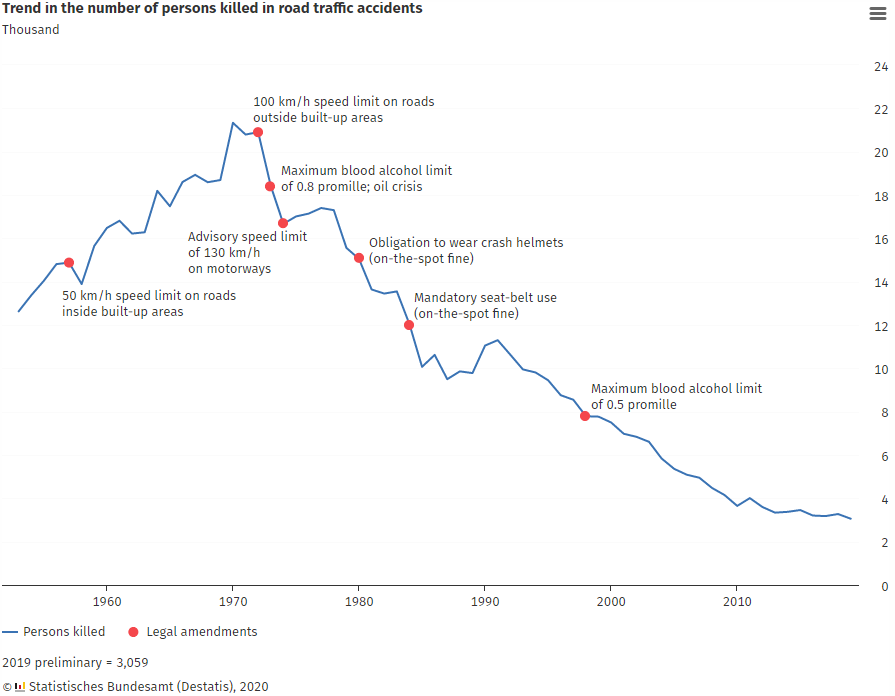
\includegraphics[width=0.9\linewidth]{chapters/chapter6_bruno/Figures/trendV2.png}
  \caption{Car Accident Trend \cite{destatisCar}}
  \label{6fig:trend}
\end{figure}

\noindent
But the decline has stagnated which still leaves around 3000 deaths a year in Germany.
Aside from the measures seen in Figure \ref{6fig:trend}, 
which try to keep accidents from happening, 
there is also another way to potentially save lives.
If the response from medical and police forces to an accident can be improved,
fewer accidents might lead to deaths. 
\\
\newline
This is what this part of the project was about. 
The goal was to connect all cars to the central server of the city.
These cars should always listen to their various sensors
and send a notification to the server
in case of an emergency.
Those emergencies are a physical crash or 
a sudden abnormality in the vitals of the driver.
\\
\newline
To simulate all this, the open source software CARLA was used.\footnote
{https://carla.org} 
CARLA is mostly used for traffic simulation and to develop autonomous driving prototypes,
but for this project, 
it served as a way to visualise the car crashes and the entire Smart City.
\\
\newline
The source code and an installation guide for this part of the project
can be found on GitHub.\footnote
{https://github.com/BrunoBerger/Connected-Vehicles}
The concept and the requirements can also be found
in the Wiki of the repository.
\section{Related Works}


\section{Concept}\label{6sec:concept}

The communication with the central server was required to be via the 
MQTT protocol for every part of the Smart City Project.
It is designed to still function even with high latency's 
and limited bandwidth, 
so its something that could also realistically be used 
in a real world implementation of a Smart City.

\noindent
As mentioned in Section \ref{6sec:intro},
CARLA was also already decided as the way to simulate the cars. 
The rest of the development of the concept was mostly driven by small experiments 
with the example scripts from the CARLA Python API. 
These covered spawning NPCs, Non-Player-Characters, 
which autonomously drive around the city,
or changing the weather in the simulation.

\noindent
The example scripts also contain a basic manually drivable car.
This car object already has multiple sensors implemented for it,
including a collision sensor.
This would provide a easy way to fulfill the crash detection part of the task
and it was then possible to write the formal requirements for the system.

\vspace{-18pt}
\subsection{Requirements}
The Requirements, as depicted in Figure \ref{6fig:reqTable}, 
were published to the Wiki of the GitHub repository on May 5th.

\noindent
In the conclusion these will be looked at again, 
to see if all requirements are satisfied by the implementation

\vspace{-4pt}
\begin{figure}[H]
  \centering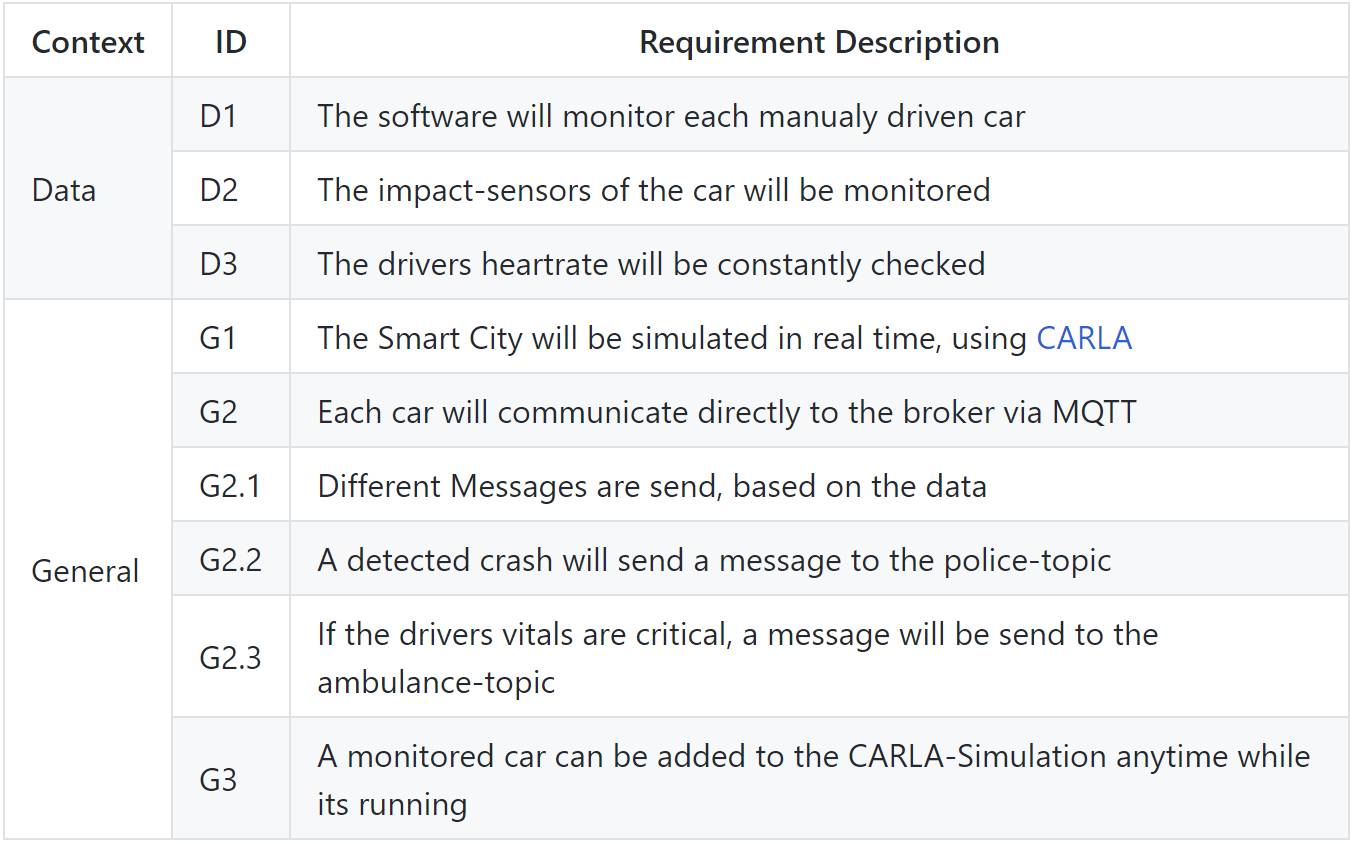
\includegraphics[width=1.0\linewidth]{chapters/chapter6_bruno/Figures/requirements.png}
  \caption{Table of requirements on GitHub}
  \label{6fig:reqTable}
\end{figure}
\vspace{-34pt}
\subsection{Sequence Chart}

\noindent
As the final part of the concept, the UML Sequence Chart seen in 
Figure \ref{6fig:sequenceChart1} was created. 
Although the exact message arguments are slightly altered in the final implementation,
The sequence of events is still the same.
Only the \emph{Driver} and the \emph{Auto} lifelines 
are actually part of this section of the project, 
but the rest also appear here,
to show how the whole Smart City works in these situations. 
\\
\newline
The first loop in Figure \ref{6fig:sequenceChart1} represents the vitals monitor 
that runs in parallel to the crash detection.
It request the heart rate from the sensor
and checks if it is outside the normal range.
If the value is dangerous, a message to the server is send,
containing information about the driver, the position of the car
and the heart rate.
The server then processes this information and sends a message to the ambulances,
but this is again, not part of this section of the project Smart City.

\begin{figure}[H]
  \centering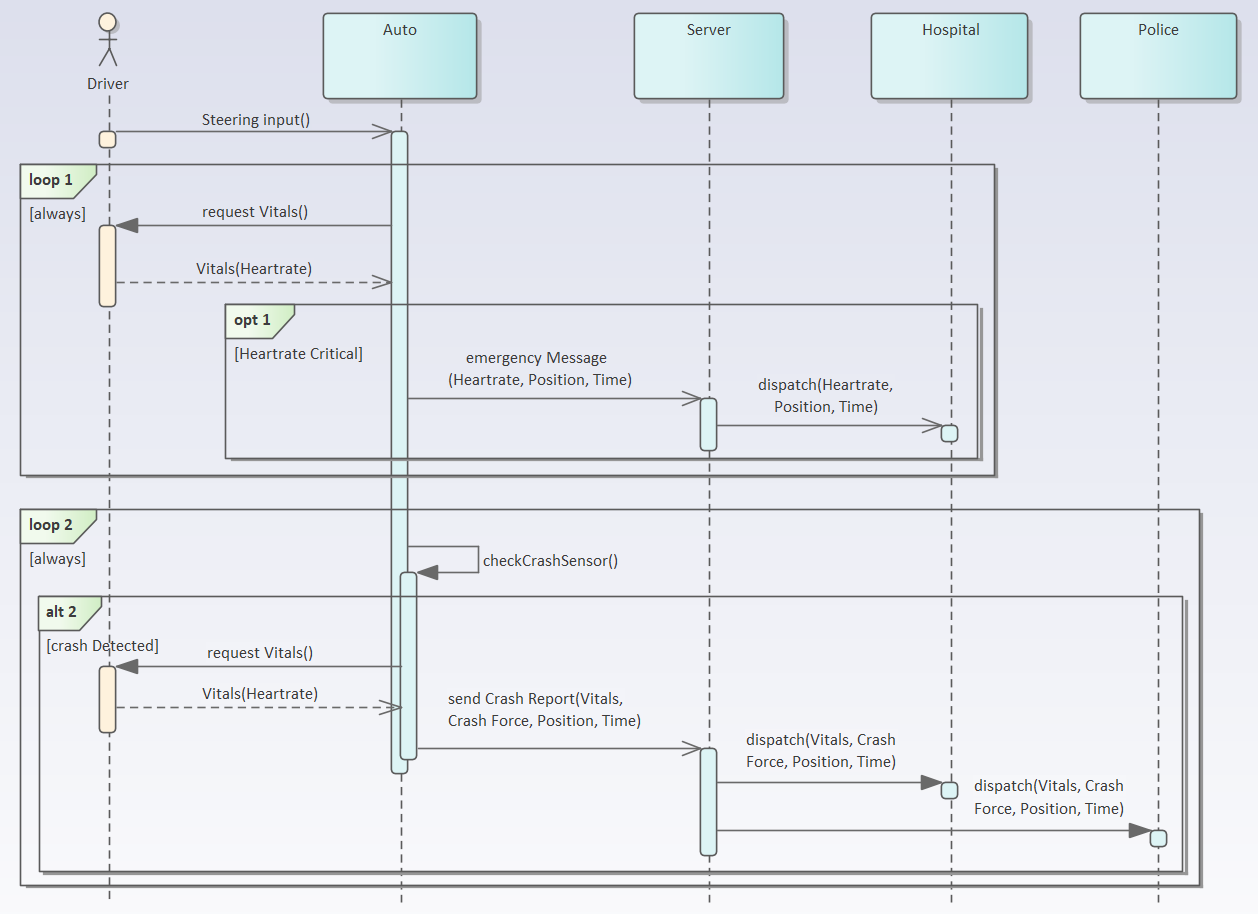
\includegraphics[width=1.0\linewidth]{chapters/chapter6_bruno/Figures/sequence1.png}
  \caption{Sequence Charts}
  \label{6fig:sequenceChart1}
\end{figure}

\noindent
The second loop shows how the crash detection works
in a very similar way.
The crash sensor is constantly monitored while the car is running.
If a collision is detected, the system gets the heart rate of the driver
and sends the message that a crash has occurred.
This message includes all known information about the crash.
If the heart rate is also critical,
a second message is send, like the one in the first loop.
\section{Implementation} \label{6sec:impl}
%   if you have class diagram
% \\ or an image that show parts of your system
% \\ screenshots of part of your code
% \\ explain the main parts of the code
% \\ make a relation between the functionalities of the system and the requirements
% \\ like: this part of the code does that which is described in the requirement FR1.

The following section will explain the general structure of the system,
as well as some important specific aspects of the implementation.
One part of the system is the CARLA simulation,
which represents the central Smart City.


% \begin{figure}[H]
%   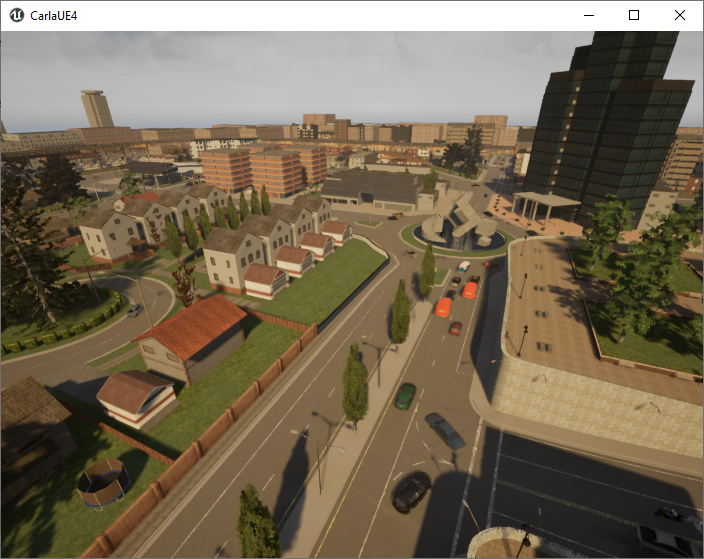
\includegraphics[width=0.6\linewidth]{chapters/chapter6_bruno/Figures/UECity1.png}
%   \caption{City rendered in Unreal Engine 4}
%   \label{6fig:cityRender}
% \end{figure}
\begin{wrapfigure}{r}{0.5\textwidth}
    \vspace{-0pt}
  \centering{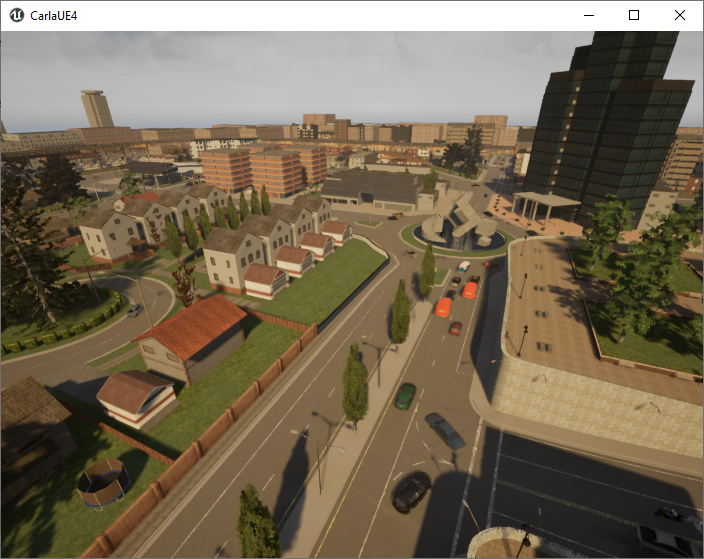
\includegraphics[width=\linewidth]{chapters/chapter6_bruno/Figures/UECity1.png}}
    \vspace{-10pt}
  \caption{City rendered in Unreal Engine 4}
  \label{6fig:cityRender}
    \vspace{-10pt}
\end{wrapfigure}

\noindent
This simulation runs independently of the rest of the project
and is also not part of the source code in this projects GitHub repository.

\noindent
It could be hosted on any cloud,
although for all tests of the project
it was running on the same PC as the crash-detection program.
\\
\newline
The simulation is running on the Unreal Engine 4 
and looks like Figure \ref{6fig:cityRender} while its online.
In this window, a flying camera can be controlled,
to watch over the city,
but a no-render mode is also available for the simulation.
There are a few different cities to load in already in CARLA,
but custom levels could also be generated.
After the crash-detection program has connected to the simulation,
in the case of the tests to the localhost,
it can intact with the simulation through the Python API from CARLA. 
\\
\newline
The starting point for the rest of the system is the \emph{main.py} file.
Here basics like ensuring the right
working directory or the command-line arguments are set up.

\begin{wrapfigure}{l}{0.4\textwidth}
    \vspace{-16pt}
  \centering{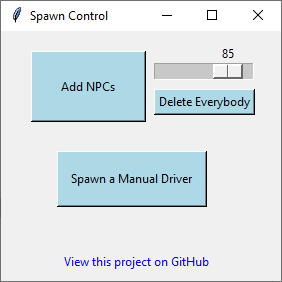
\includegraphics[width=\linewidth]{chapters/chapter6_bruno/Figures/ui1.png}}
    \vspace{-10pt}
  \caption{Tkinter window}
  \label{6fig:ui}
    \vspace{-10pt}
\end{wrapfigure}

\noindent
After that, the window seen in Figure \ref{6fig:ui} is initialised.
For this, the package Tkinter was used.
This is the center for all action from the user.
They can add an adjustable number of NPCs to the simulation or delete all of them. 
These will drive autonomously around the town, as can be seen in Figure \ref{6fig:cityRender}.
They serve mostly as obstacles to crash into and have no further functionality to them.

\noindent
The process of actually spawning the cars into the simulation
is handled by one of the example scripts from the Python API,
\emph{spawn\_npc.py}.
\\
\newline
The framework for the manual driver is also mostly 
from the example script \emph{manual\_control.py}.
The following section will still though go over the basic principle behind it
and then explain when new features were added for this project.

\subsection{Manual Driver}\label{6sec:manCar}
\noindent
When the \emph{Spawn a Manual Driver} Button in Figure \ref{6fig:ui} is pressed,
a new thread is started, using the multiprocessing package.
This thread then executes the above mentioned script.
Using threading means that the user can generate as many manual drivers as they want,
only being limited by their system resources.

\noindent
At the start of the script,
a connection to the MQTT server was added.
The each manual car is given a random name from a list 
and a random ID to identify them. 
This driver is then registered on the server,
with a message with an empty reason and all information on the driver.

\noindent
After that the heart monitor was added.
It is started as a new thread, always running in the background 
of every active manual car. 
As a simulation of a real pulse sensor,
it generates a random number of a normal curve every second.

Then the code of the example script is executed. 
It first connects to the simulation,
which was running on the localhost for all tests.
Then a drivable car is created, via the "blueprints" provided by CARLA.
This car then gets sensors attached, also from blueprints.
In a final loop the window depicted in Figure \ref{6fig:manCar} is rendered,
with a few HUD elements and a camera following the car. 
The user can now control the car using the arrow-keys on the keyboard.

\begin{figure}[H]
  \centering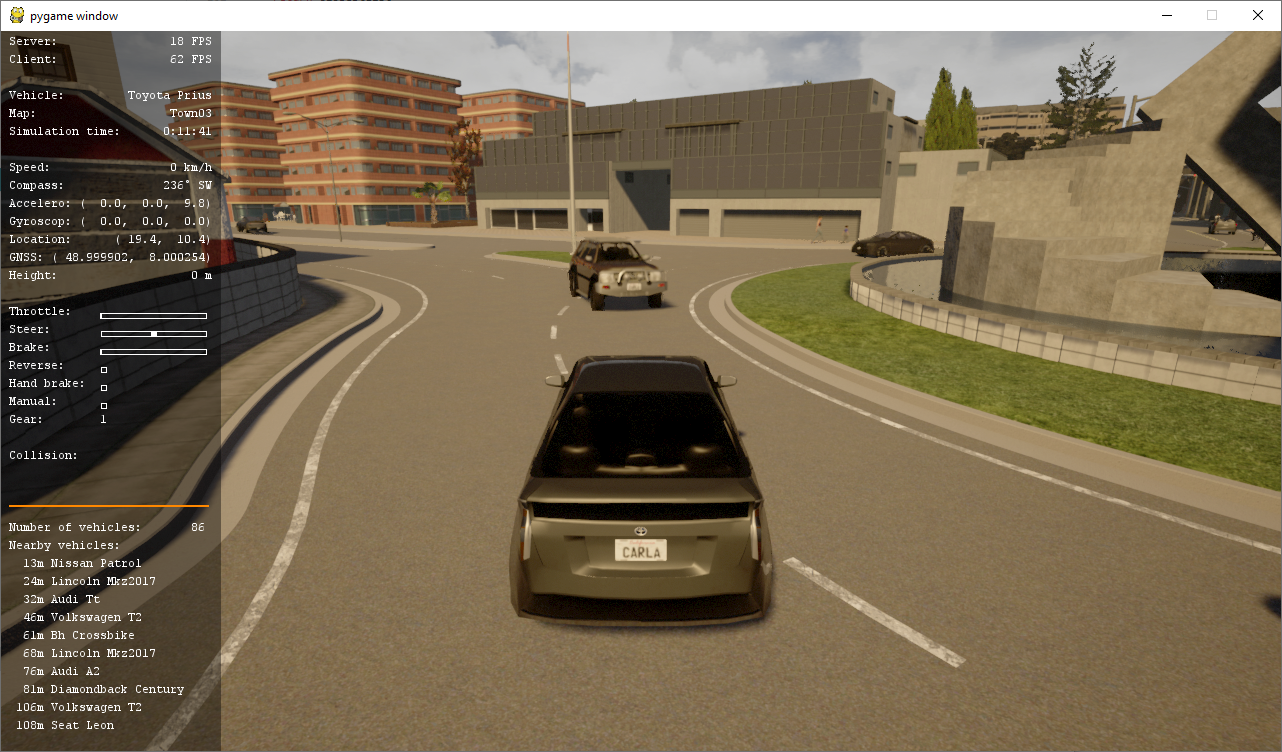
\includegraphics[width=0.9\linewidth]{chapters/chapter6_bruno/Figures/manual1.png}
  \caption{Manually Controllable Car}
  \label{6fig:manCar}
\end{figure}

\noindent
As mentioned, these cars have a collision sensor.
This sensor is continually listening to a \emph{\_oncollision\_()} method. 
This made it very easy to implement the concept of monitoring crashes.

\begin{wrapfigure}{l}{0.55\textwidth}
    \vspace{-16pt}
  \centering{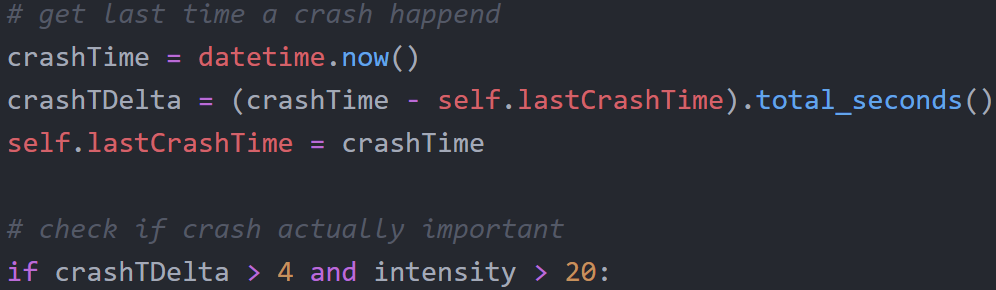
\includegraphics[width=\linewidth]{chapters/chapter6_bruno/Figures/collisionCode.png}}
    \vspace{-16pt}
  \caption{Time and force filter}
  \label{6fig:onCollCode}
    \vspace{-18pt}
\end{wrapfigure}

\noindent
First a filter was added, seen in Figure \ref{6fig:onCollCode},
which checks the validity of the crash.
The timestamp of the crash is compared to the one of the last registered crash.
Then, if the this last crash didn't happen in the last 4 seconds
and if the intensity of the collision is high enough,
the emergency message will be generated (Figure \ref{6fig:onCollCode2}).

\noindent
This filter ensures two things.
A single car crash could consist of multiple impacts in quick succession,
which would otherwise all activate their own messages.
It also removes false positives, from small impacts
like a speed bump.
\begin{wrapfigure}{l}{0.55\textwidth}
    \vspace{-6pt}
  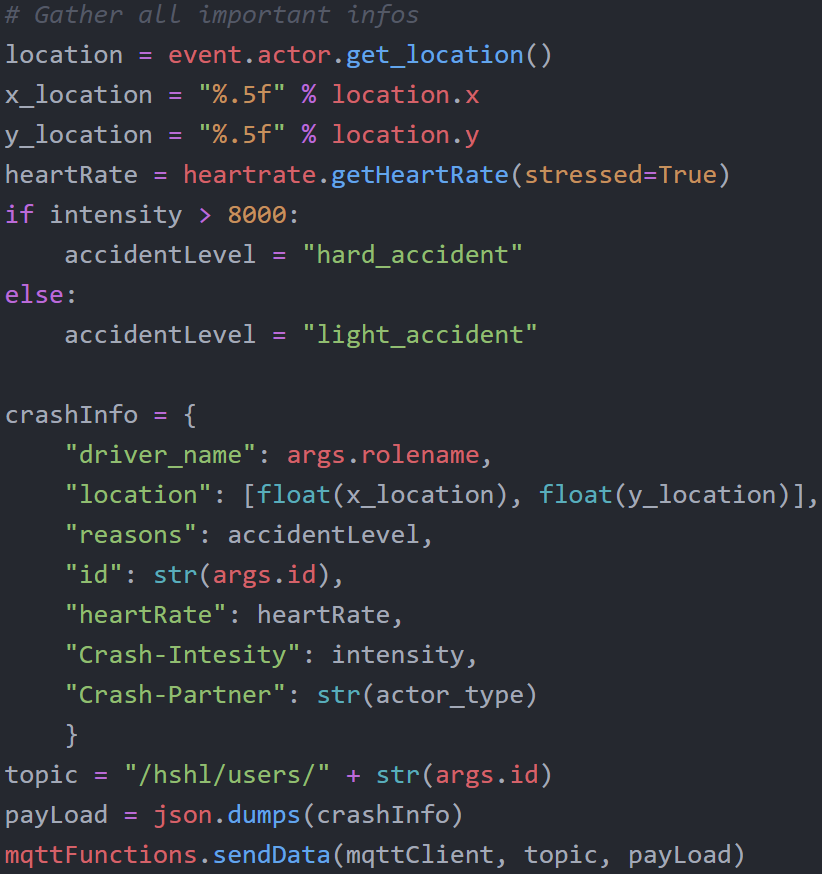
\includegraphics[width=\linewidth]{chapters/chapter6_bruno/Figures/collisionCode2.png}
    \vspace{-10pt}
  \caption{Message Generation}
  \label{6fig:onCollCode2}
  \vspace{-20pt}
\end{wrapfigure}
\\
\noindent
If the crash is validated, additional information on the crash is gathered,
as can be seen at the top of Figure \ref{6fig:onCollCode2}.
Its also decided whether to classify the crash as a hard or a light one,
which could potentially change the reaction from the server.
\\
\newline
Finally, all relevant information gets stored as a json dump,
which converts them into a long string that is compatible with the MQTT protocol.
The message is then send to the specific topic of the driver.\linebreak

\noindent
After that the system the checks if the heart rate of the driver is critical.
If so, a second, slightly different message will be created and send.
It only contains the basic driver information and
is intended to be forwarded to the ambulances of the city.

\noindent
This is done to fulfill the requirements G2.2 and G2.3.
Those were created when the concept of the server wasn't final yet
and were intended for a slightly different message handling structure.
This system is still fully functional,
but the second message is not really needed today.


\section{Conclusion}

\subsection{Results}\label{6sec:Results}
%   show what is working
% \\ which requirements are not implemented?
% \\ what could you have done in a different way?

The implementation works as it should.
The user can add add or remove as many NPCs or manual drivers as they want.
All requirements are fulfilled in the final version,
with the caveat mentioned above in Section \ref{6sec:manCar}.
When a manual driver crashes into something, 
the messages are successfully send to the MQTT server.
The filter also works well, 
though it could be argued that the strict four 
second threshold is too simplistic.

\noindent 
There is at the time of writing a problem with the communication with the server,
where the accident reports are not correctly registered.
But this seems to be a relatively simple matter 
of getting the right formatting,
either on the server or the client end.
But overall, the goal of creating a smart city 
that monitors the car safety of its citizens has been achieved.

\subsection{Future work}\label{6sec:future Work}

Currently a lot of information is send to the server that is completely ignored.
Values like the heart rate, the intensity of the crash
or the object that the car crashed into.
Further functionality could be added to the server and
the ambulance projects, to take these into account.
This could help make better decisions in cases 
where there is a high demand for emergency responses,
but not enough capacity a the facilities.

To the crash detection program, a feature to detect if the crash partner is also 
a manual car could be added.
This could make it so that only one emergency message is send to the hospital,
not two for the same crash.
\\
\newline
The biggest improvement to the system  would be to and the crash monitoring to NPCs.
This could make this project a true simulation of a smart city,
when the system doesn't require a user to crash Manual Cars into walls.
To push the total simulation thought even further,
the hospitals could also be implemented in CARLA,
so the ambulances actually respond to the message and drive to the location.


%\newpage
\bibliographystyle{IEEEtran}
\bibliography{chapter6.bib}

\chapter{User in Smart Cities and new HMI}
\label{intro} 


\abstract{
\\ (1 or 2 lines): Give a context of your project
\\(1 line): what is the problem?
\\(2 lines): how are you solving it?
\\(1 or 2): what are the results/conclusions
}

\section{Introduction}
\label{sec:1}


\section{Related works}
\label{sec:2}

The research group BLABLA \cite{cheng2015building} did a similar work....using MQTT as it is shown in Figure \ref{fig:1}.
\begin{figure}
\sidecaption
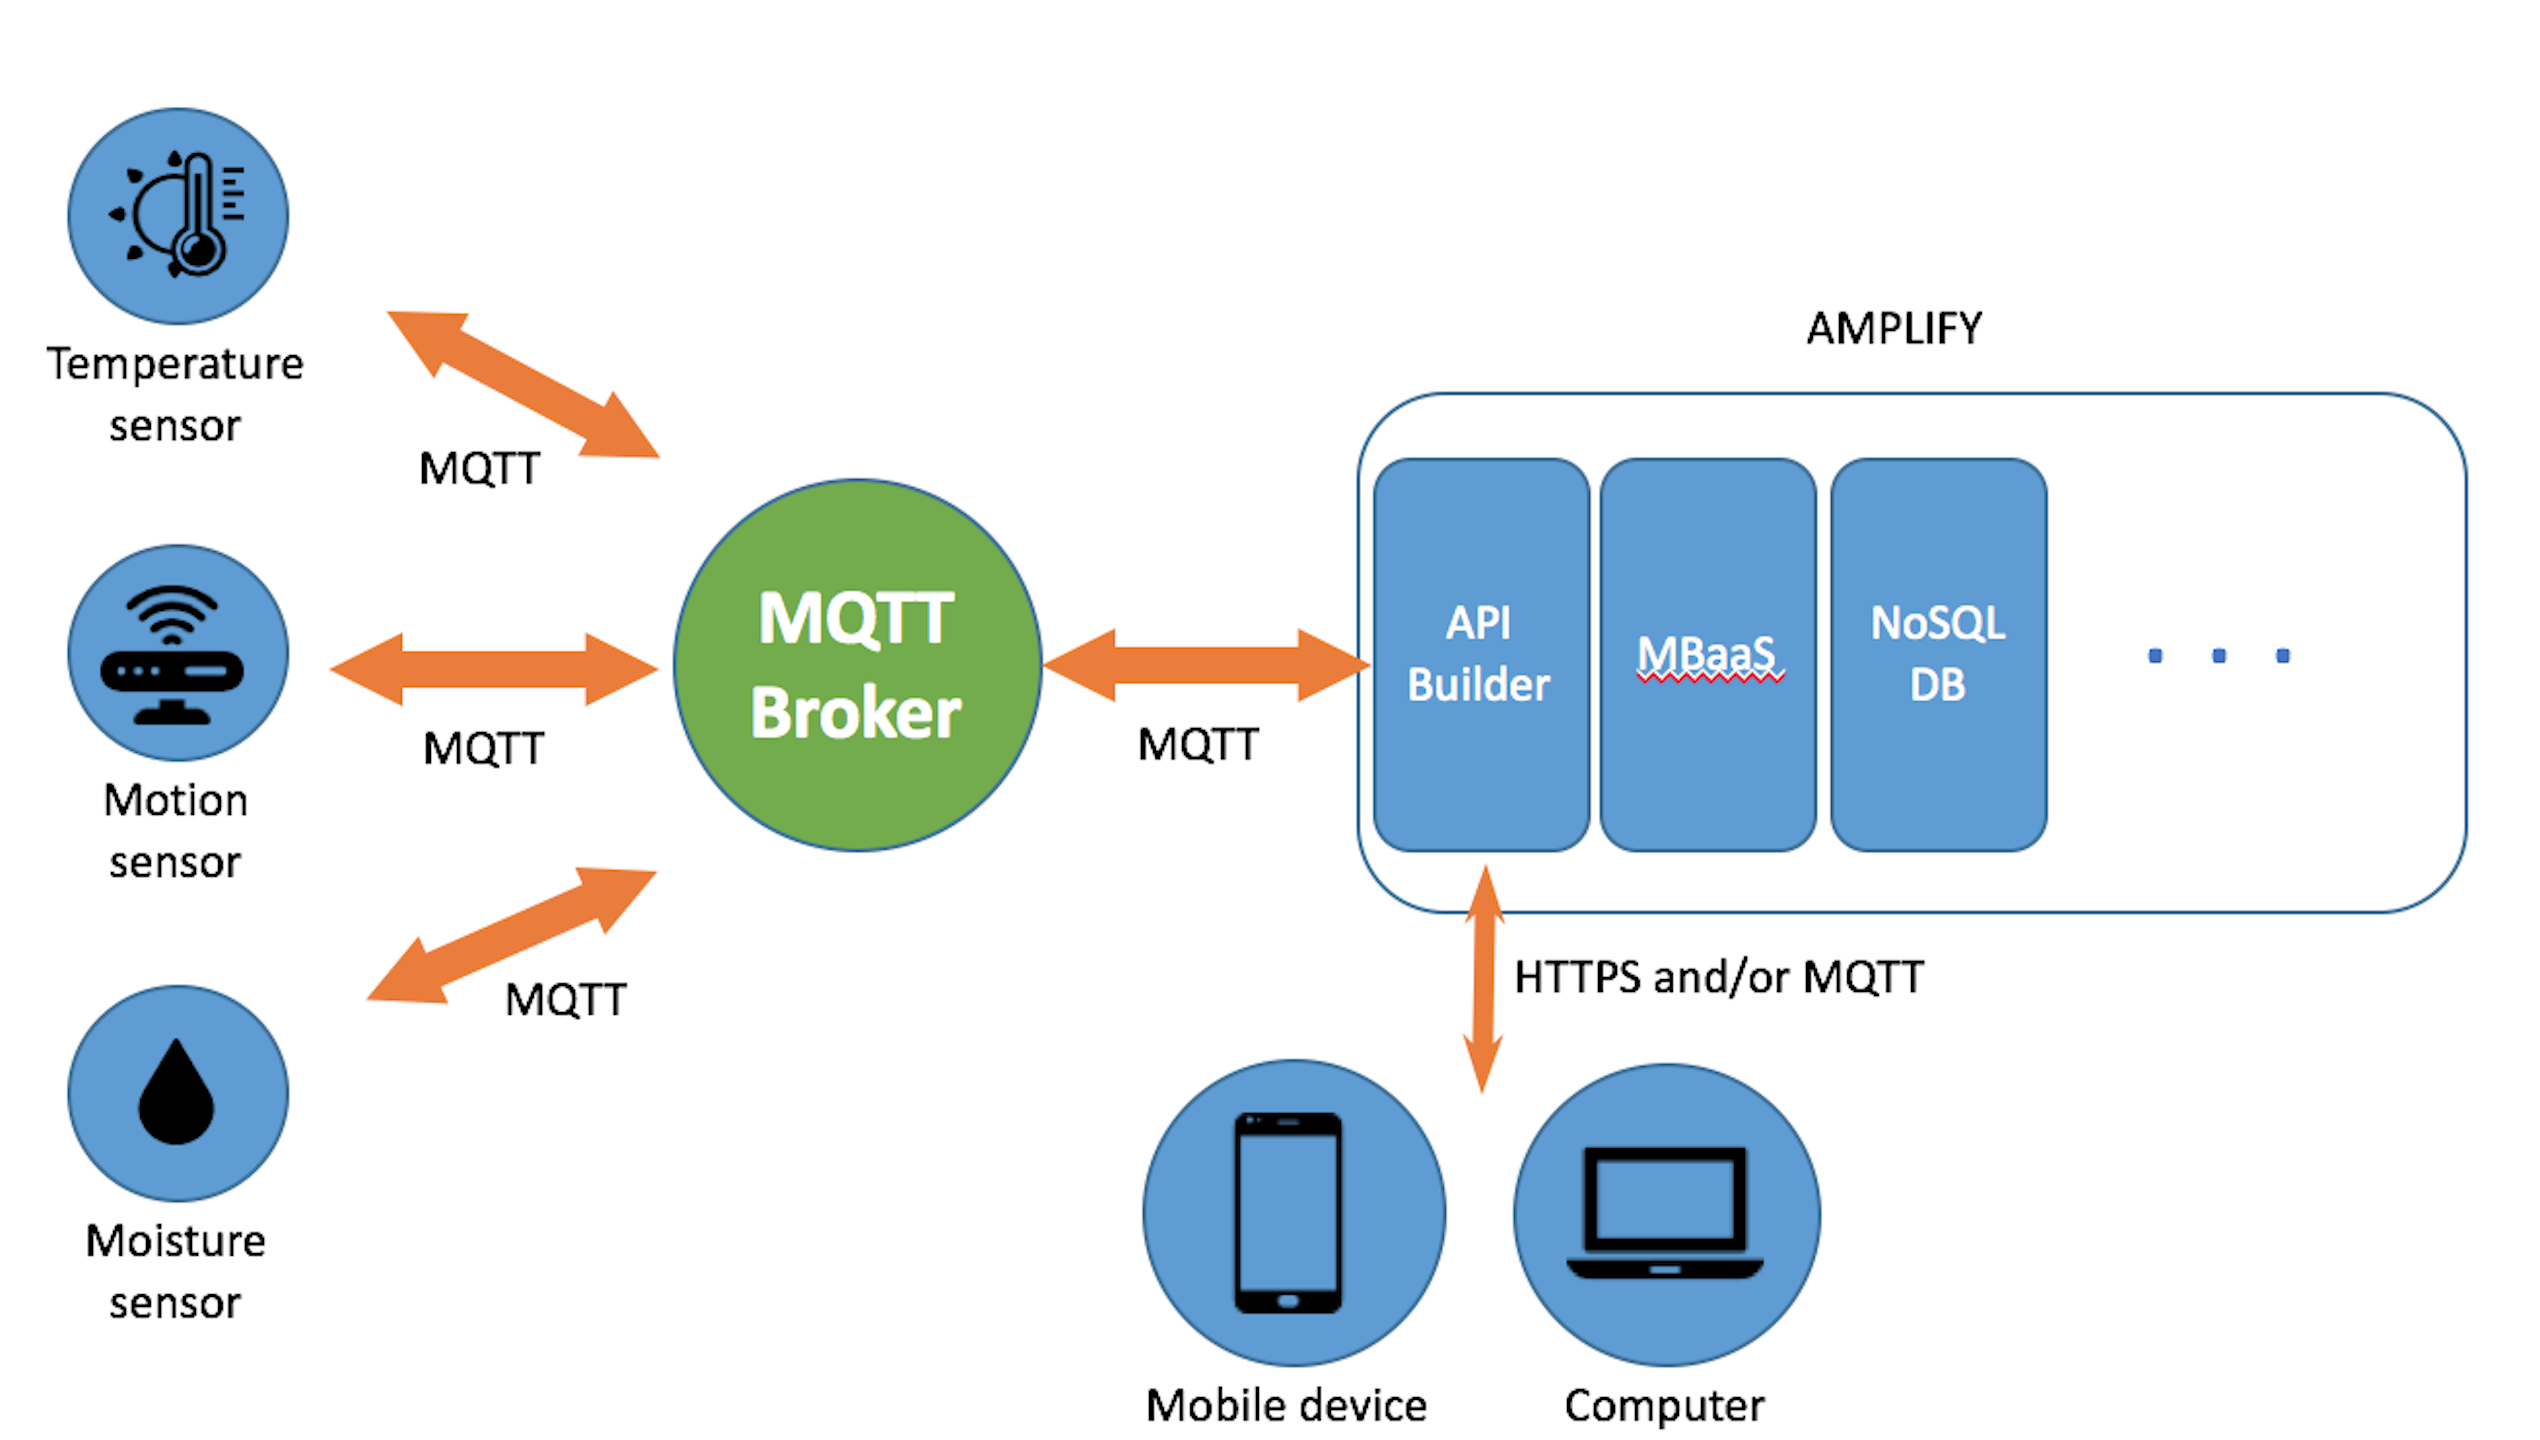
\includegraphics[scale=.09]{images/figure.png}
\caption{this is a picture}
\label{fig:1}
\end{figure}


\section{Your proposal (Concept)}
\label{sec:3}
   What is your project?
\\ requirements table
\\ Add a picture explaining how it works (concept)
\\ Diagrams
\\

\section{Implementation of your proposal}
\label{sec:4}
   if you have class diagram
\\ or an image that show parts of your system
\\ screenshots of part of your code
\\ explain the main parts of the code
\\ make a relation between the functionalities of the system and the requirements
\\ like: this part of the code does that which is described in the requirement FR1.

\section{Results}
\label{sec:5}
   show what is working
\\ which requirements are not implemented?
\\ what could you have done in a different way?

\section{Conclusion}
\label{sec:5}
...
\\ future work
\chapter{MQTT Broker redundancy}
\label{intro} 


\abstract{
\\ (1 or 2 lines): Give a context of your project
\\(1 line): what is the problem?
\\(2 lines): how are you solving it?
\\(1 or 2): what are the results/conclusions
}

\section{Introduction}
\label{sec:1}


\section{Related works}
\label{sec:2}

The research group BLABLA \cite{cheng2015building} did a similar work....using MQTT as it is shown in Figure \ref{fig:1}.
\begin{figure}
\sidecaption
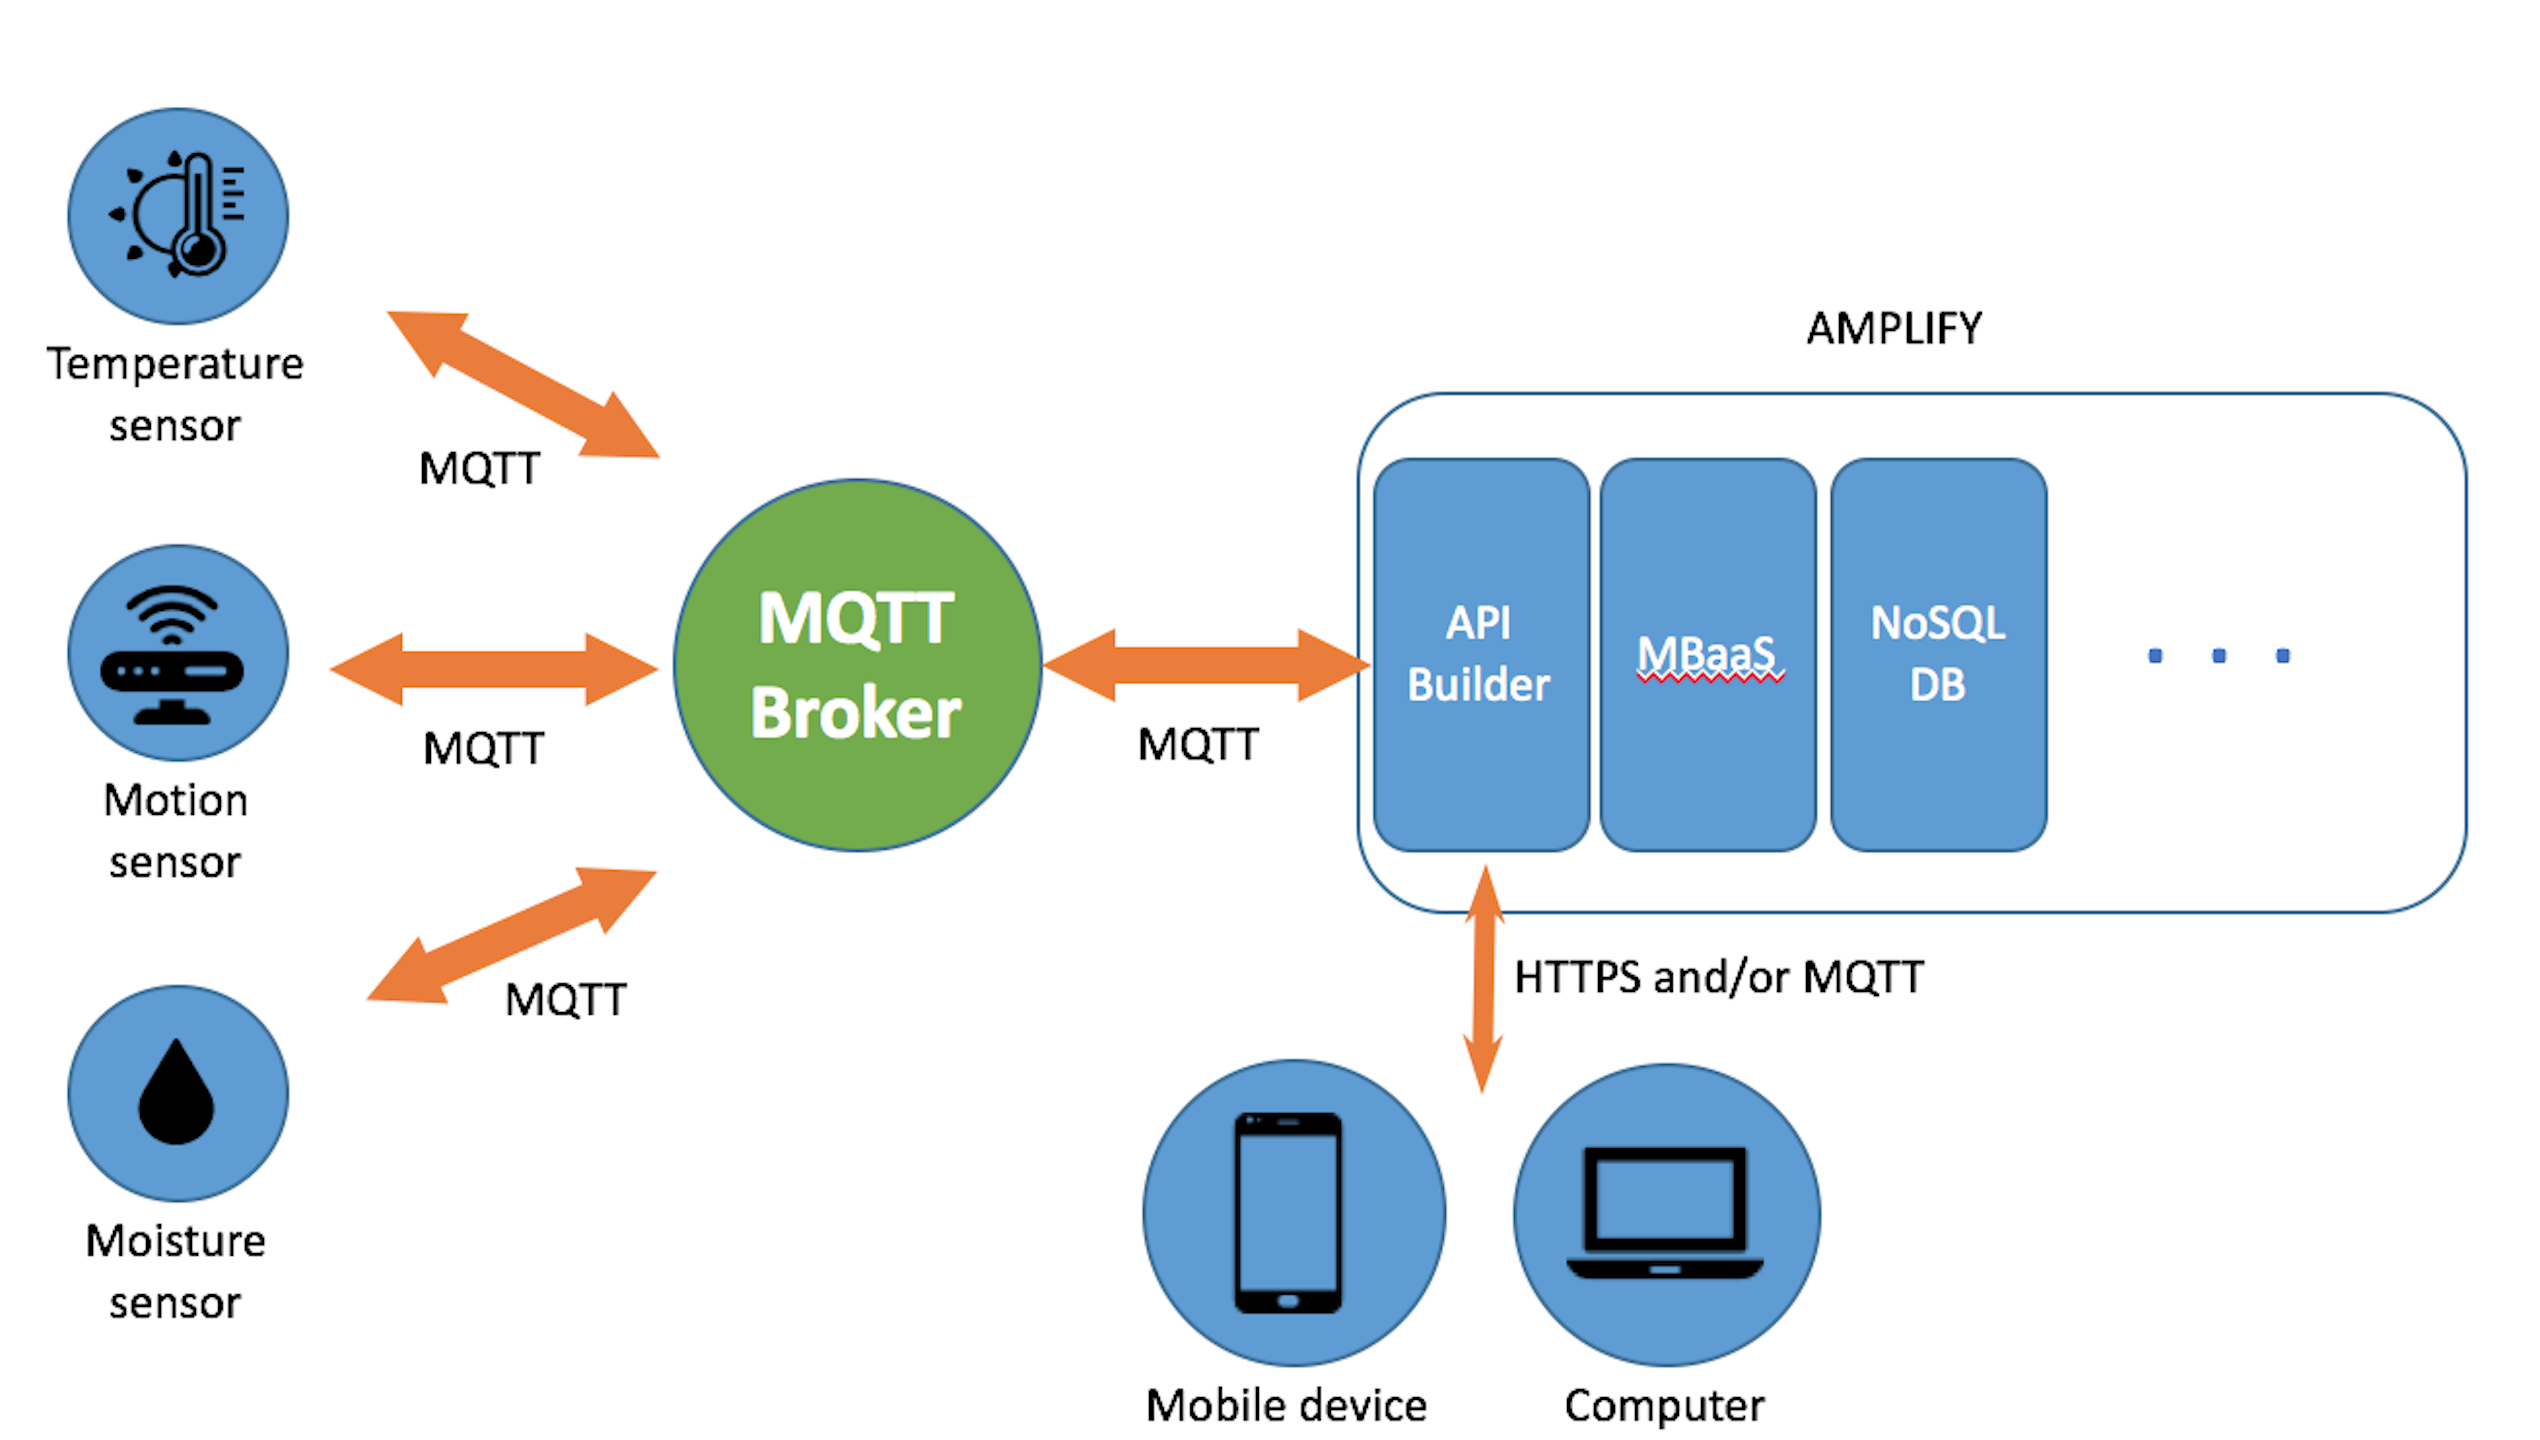
\includegraphics[scale=.09]{images/figure.png}
\caption{this is a picture}
\label{fig:1}
\end{figure}


\section{Your proposal (Concept)}
\label{sec:3}
   What is your project?
\\ requirements table
\\ Add a picture explaining how it works (concept)
\\ Diagrams
\\

\section{Implementation of your proposal}
\label{sec:4}
   if you have class diagram
\\ or an image that show parts of your system
\\ screenshots of part of your code
\\ explain the main parts of the code
\\ make a relation between the functionalities of the system and the requirements
\\ like: this part of the code does that which is described in the requirement FR1.

\section{Results}
\label{sec:5}
   show what is working
\\ which requirements are not implemented?
\\ what could you have done in a different way?

\section{Conclusion}
\label{sec:5}
...
\\ future work

\newpage
\bibliographystyle{IEEEtran}
\bibliography{./chapter.bib}
\chapter{HMI tracking}
\label{intro} 


\abstract{
\\ (1 or 2 lines): Give a context of your project
\\(1 line): what is the problem?
\\(2 lines): how are you solving it?
\\(1 or 2): what are the results/conclusions
}

\section{Introduction}
\label{sec:1}


\section{Related works}
\label{sec:2}

The research group BLABLA \cite{cheng2015building} did a similar work....using MQTT as it is shown in Figure \ref{fig:1}.
\begin{figure}
\sidecaption
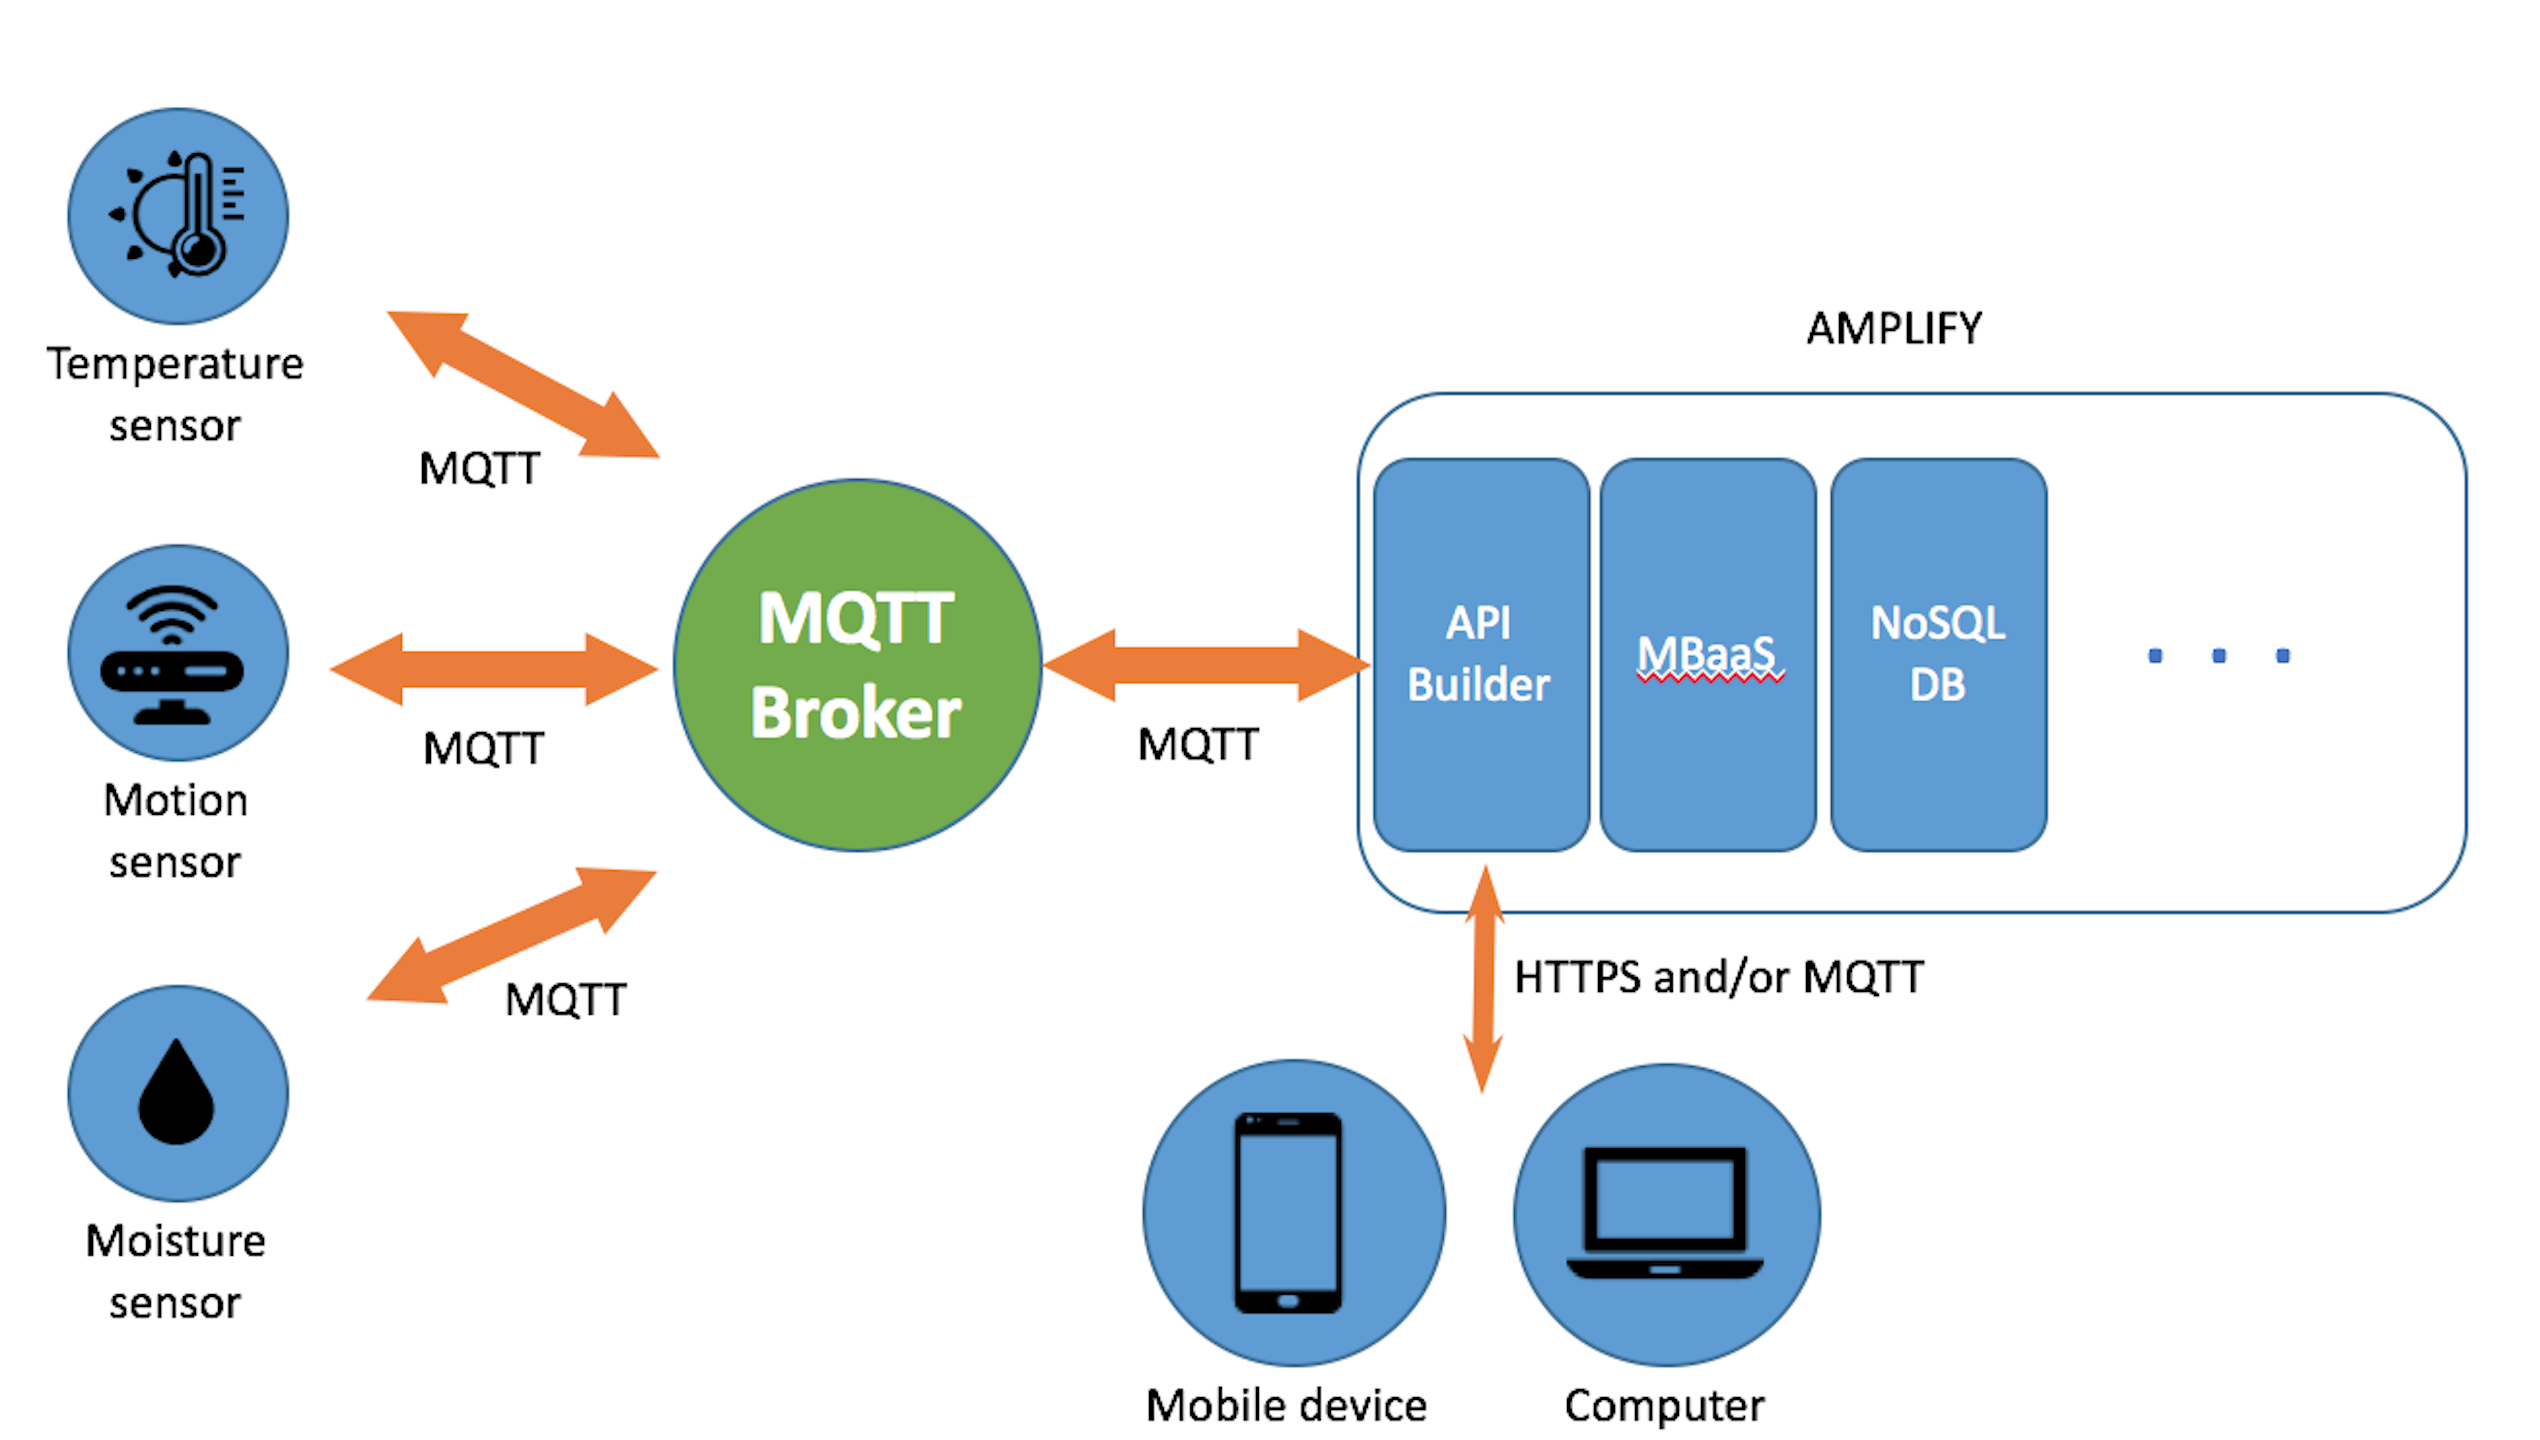
\includegraphics[scale=.09]{images/figure.png}
\caption{this is a picture}
\label{fig:1}
\end{figure}


\section{Your proposal (Concept)}
\label{sec:3}
   What is your project?
\\ requirements table
\\ Add a picture explaining how it works (concept)
\\ Diagrams
\\

\section{Implementation of your proposal}
\label{sec:4}
   if you have class diagram
\\ or an image that show parts of your system
\\ screenshots of part of your code
\\ explain the main parts of the code
\\ make a relation between the functionalities of the system and the requirements
\\ like: this part of the code does that which is described in the requirement FR1.

\section{Results}
\label{sec:5}
   show what is working
\\ which requirements are not implemented?
\\ what could you have done in a different way?

\section{Conclusion}
\label{sec:5}
...
\\ future work
\chapter{Human Machine Interface tracking}
\label{intro} 


\abstract{
\\ (1 or 2 lines): Give a context of your project
\\(1 line): what is the problem?
\\(2 lines): how are you solving it?
\\(1 or 2): what are the results/conclusions
}

\section{Introduction}
\label{sec:1}


\section{Related works}
\label{sec:2}

The research group BLABLA \cite{cheng2015building} did a similar work....using MQTT as it is shown in Figure \ref{fig:1}.
\begin{figure}
\sidecaption
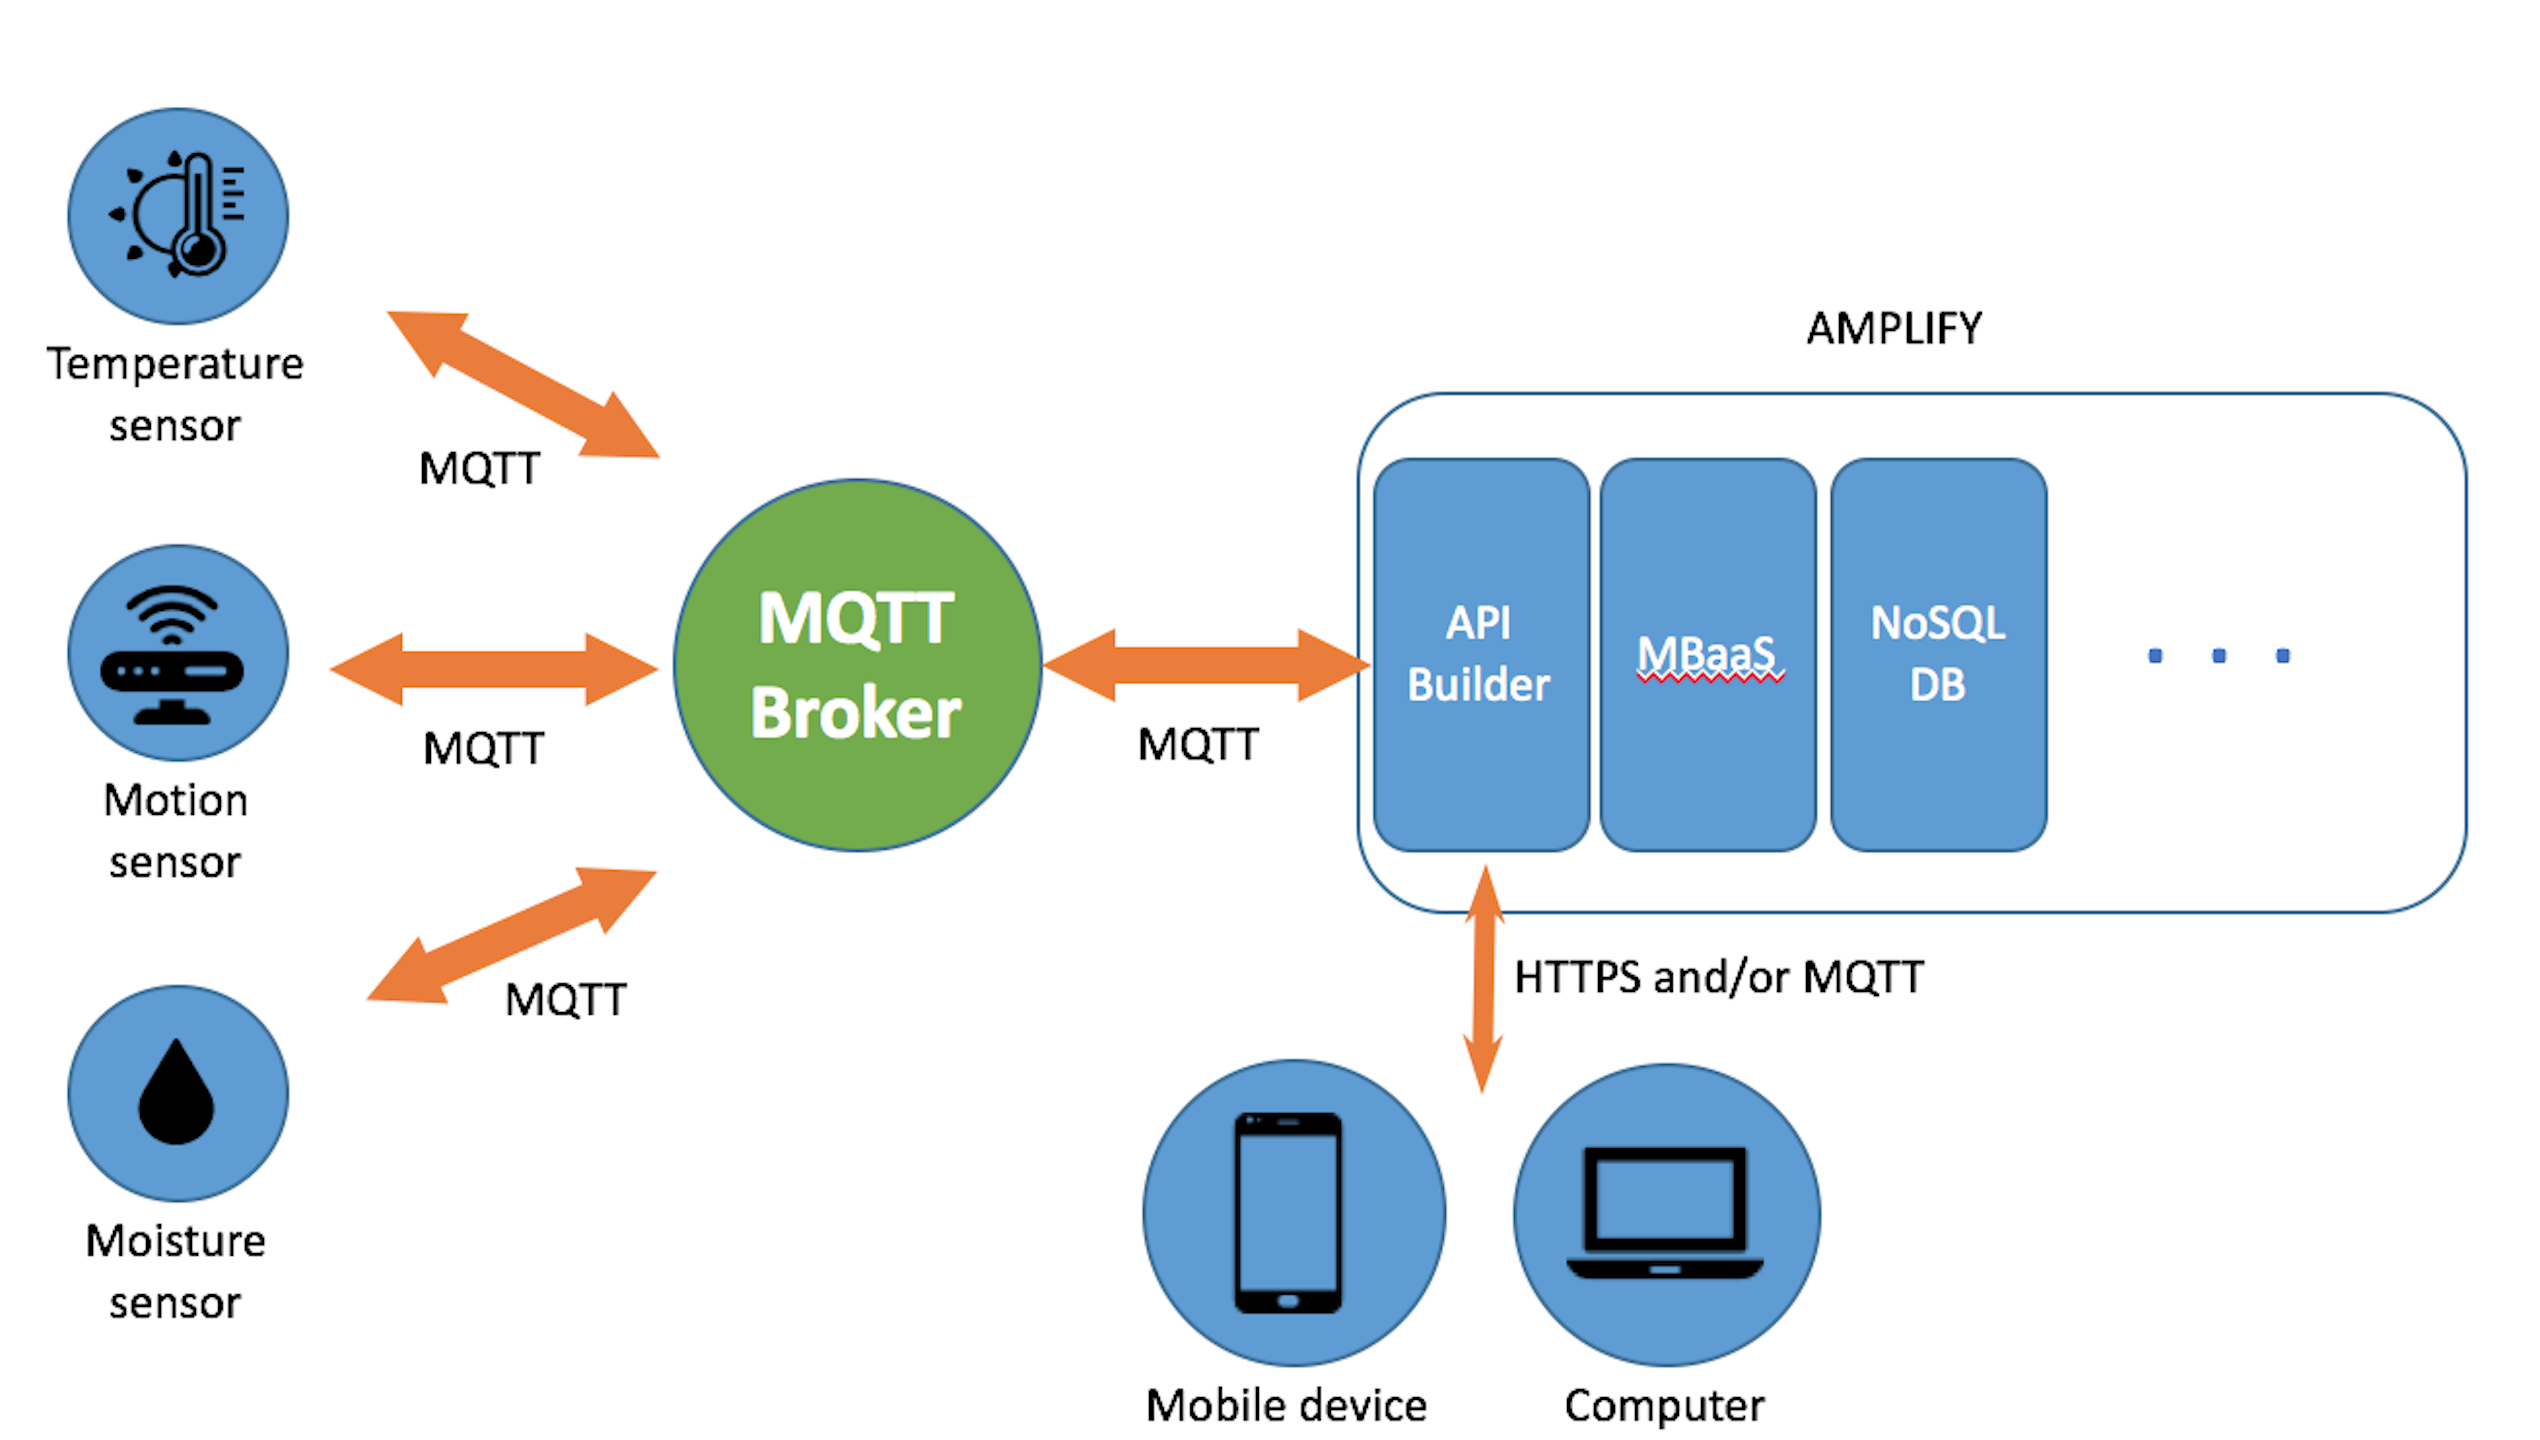
\includegraphics[scale=.09]{images/figure.png}
\caption{this is a picture}
\label{fig:1}
\end{figure}


\section{Your proposal (Concept)}
\label{sec:3}
   What is your project?
\\ requirements table
\\ Add a picture explaining how it works (concept)
\\ Diagrams
\\

\section{Implementation of your proposal}
\label{sec:4}
   if you have class diagram
\\ or an image that show parts of your system
\\ screenshots of part of your code
\\ explain the main parts of the code
\\ make a relation between the functionalities of the system and the requirements
\\ like: this part of the code does that which is described in the requirement FR1.

\section{Results}
\label{sec:5}
   show what is working
\\ which requirements are not implemented?
\\ what could you have done in a different way?

\section{Conclusion}
\label{sec:5}
...
\\ future work

\newpage
\bibliographystyle{IEEEtran}
\bibliography{./chapter.bib}

\backmatter%%%%%%%%%%%%%%%%%%%%%%%%%%%%%%%%%%%%%%%%%%%%%%%%%%%%%%%
\printindex

%%%%%%%%%%%%%%%%%%%%%%%%%%%%%%%%%%%%%%%%%%%%%%%%%%%%%%%%%%%%%%%%%%%%%%

\end{document}





